\thispagestyle{thachthuctoanhocnone}
\pagestyle{thachthuctoanhoc}
\everymath{\color{thachthuctoanhoc}}
\graphicspath{{../thachthuctoanhoc/pic/}}
\begingroup
\AddToShipoutPicture*{\put(0,616){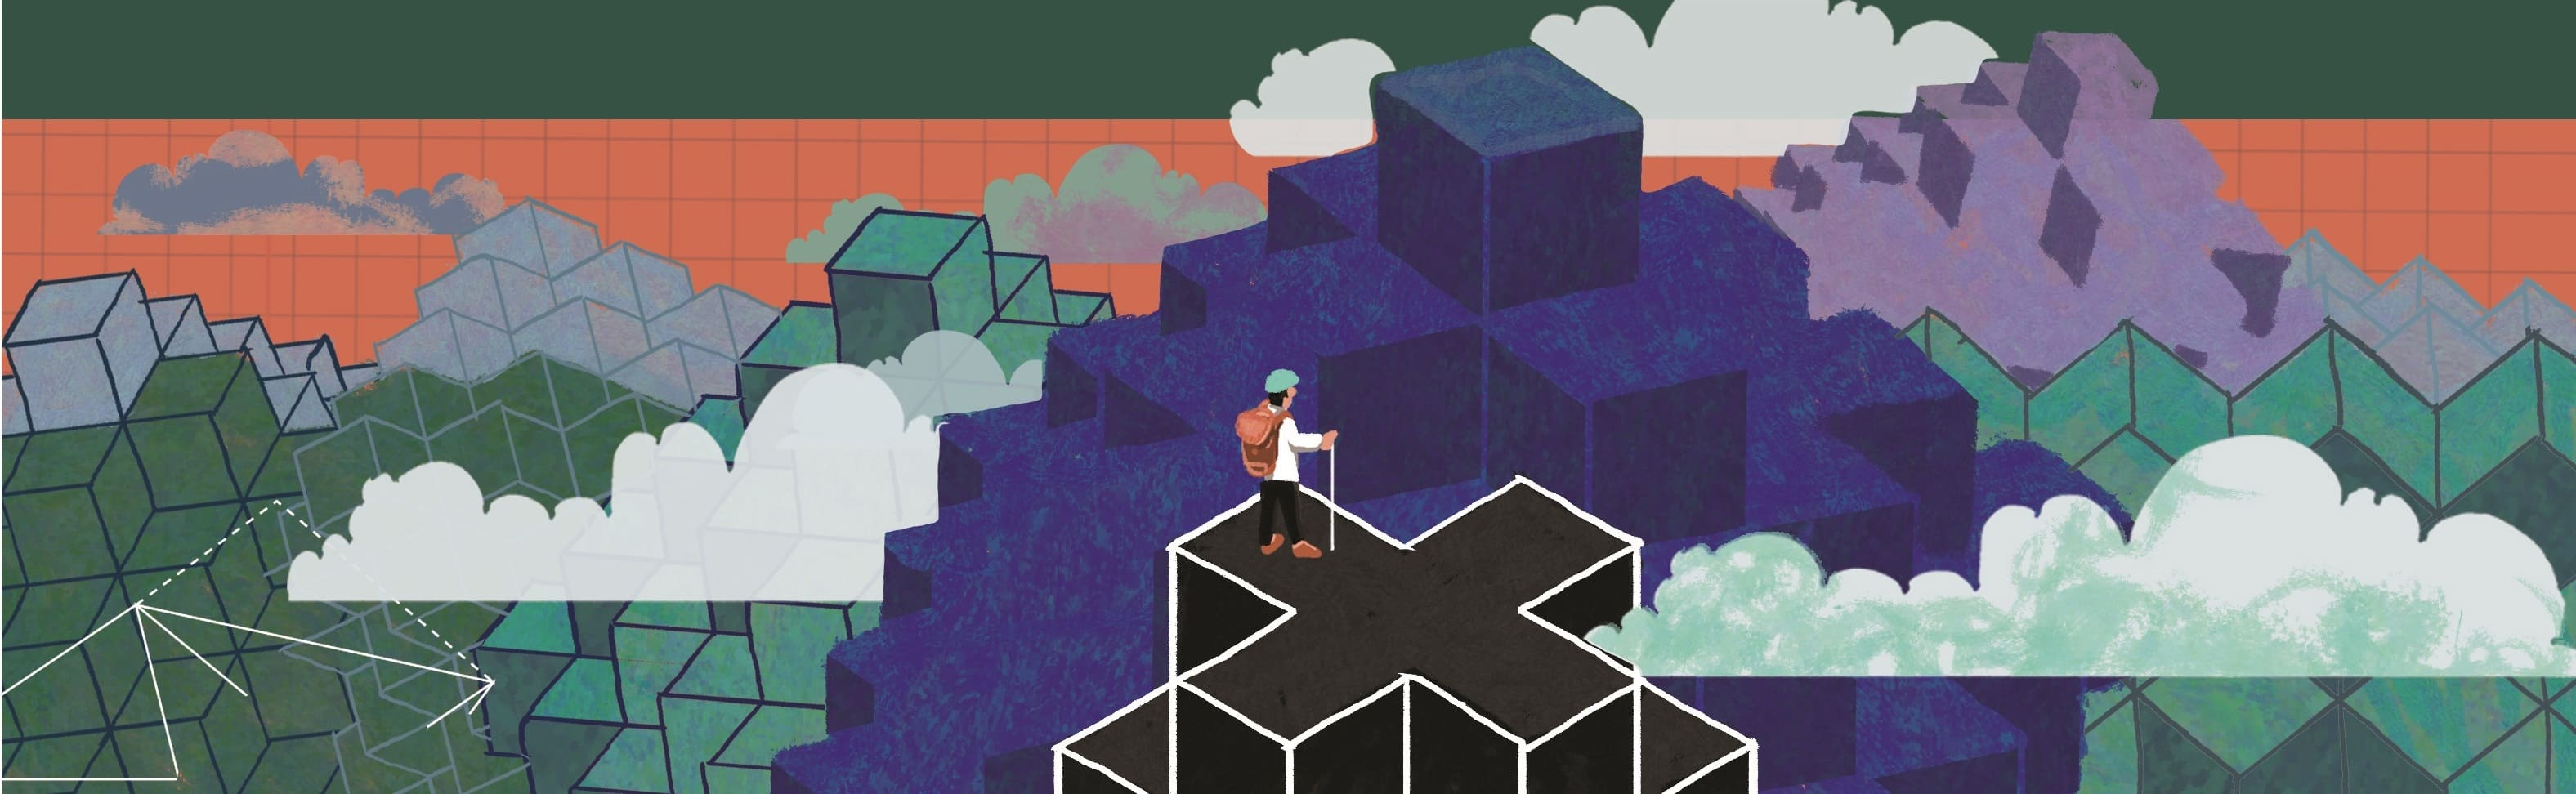
\includegraphics[width=19.3cm]{../thachthuctoanhoc/bannerthachthuc}}}
\centering
\vspace*{4cm}
\endgroup
\vspace*{-8pt}
\begin{tBox}
	\begin{itemize}[leftmargin = 13pt, itemsep = 1.0pt] 
				\item Mỗi bài toán đề xuất (kèm theo lời giải) cần được nêu rõ là bài sáng tác hay bài sưu tầm.
%		\item Mỗi bài toán đề xuất (kèm theo lời giải) cần được nêu rõ là bài sáng tác hay bài sưu tầm (nếu là bài sưu tầm, cần ghi rõ nguồn).
		\item Bài giải cho mỗi bài toán cần được trình bày trong một file riêng hoặc
		một tờ giấy riêng.
		\item  Người đề xuất bài toán hoặc gửi bài giải cho các bài toán trong mục ``Thách thức kỳ này" cần ghi rõ họ, đệm, tên và nơi làm việc/học tập, số điện thoại liên hệ. Nếu là học sinh (hoặc sinh viên) cần ghi rõ là học sinh lớp mấy (hoặc sinh viên năm thứ mấy).
		\item Các bài toán trong mục Thách thức kỳ này hướng tới các độc giả là học sinh phổ thông; được phân chia thành các mức độ $B$, $A$, và được sắp xếp theo độ khó tăng dần, theo đánh giá chủ quan của Ban biên tập. Các bài toán mức độ $B$ không đòi hỏi các kiến thức vượt quá chương trình môn Toán cấp THCS; các bài toán mức độ $A$ không đòi hỏi các kiến thức vượt quá chương trình môn Toán cấp THPT.
		\item Cách thức gửi bài toán đề xuất hoặc lời giải: gửi file thu được bằng cách scan, ảnh chụp (rõ nét) của bản viết tay, hoặc được soạn thảo bằng các phần mềm Latex, Word tới \url{bbt@pi.edu.vn} hoặc gửi qua đường bưu điện tới Tòa soạn (xem địa chỉ tại bìa $2$).
		\item Hạn gửi lời giải cho các bài toán P$641$--P$650$: trước ngày $15/11/2022$.
	\end{itemize}
\end{tBox}
\begin{center}
	\vspace*{-5pt}
	\textbf{\color{thachthuctoanhoc}\color{thachthuctoanhoc}THÁCH THỨC KỲ NÀY}
	\vspace*{-5pt}
\end{center}
\begin{multicols}{2}
	\setlength{\abovedisplayskip}{4pt}
	\setlength{\belowdisplayskip}{4pt}
	{\color{thachthuctoanhoc}{\usefont{T5}{qag}{b}{n} P641.}}
	(Mức $B$) Tại mỗi đỉnh của một đa giác lồi $18$ cạnh ở Hình dưới đây, người ta ghi một số, sao cho số được ghi ở mỗi đỉnh bằng tổng hai số được ghi ở hai đỉnh kề với nó.
	\begin{figure}[H]
		\vspace*{-5pt}
		\centering
		\captionsetup{labelformat= empty, justification=centering}
		\definecolor{ffvvqq}{rgb}{1,0.3333333333333333,0}
		\definecolor{qqqqffa}{rgb}{0,0,1}
		\definecolor{qqzzff}{rgb}{0,0.6,1}
		\begin{tikzpicture}[line cap=round,line join=round,>=triangle 45,x=1cm,y=1cm,scale=0.42]
			\draw (1.401115339869085,5.50644760016908136) node[anchor=north west] {$X$};
			\draw (1.4408759814898973,-0.7306378725360659) node[anchor=north west] {$Y$};
			\draw (-7.8444170535279,2.5008856260029945) node[anchor=north west] {$S$};
			\draw [color=qqzzff] (0.0915547437082469,-1.9784020259611625)--(1.3147607160299626,-0.9781184915188108);
			\draw [color=qqzzff] (1.3147607160299626,-0.9781184915188108)--(2.122081224105652,0.3802016464606015); 
			\draw [color=qqzzff] (2.122081224105652,0.3802016464606015)--(2.4161414998796458,1.932724932666551); 
			\draw [color=qqzzff] (2.4161414998796458,1.932724932666551)--(2.1614735342261406,3.4921941459791768);
			\draw [color=qqzzff] (2.1614735342261406,3.4921941459791768)--(1.38879404230183,4.87051428395859);
			\draw [color=qqzzff] (1.38879404230183,4.87051428395859)--(0.19129957436757605,5.901439596125702);
			\draw [color=qqzzff] (0.19129957436757605,5.901439596125702)--(-1.2865743636076452,6.4606252749959765);
			\draw [color=qqzzff] (-1.2865743636076452,6.4606252749959765)--(-2.866574363607645,6.480625274995977);
			\draw [color=qqzzff] (-2.866574363607645,6.480625274995977)--(-4.358129107315893,5.959027300957139);
			\draw [color=qqzzff] (-4.358129107315893,5.959027300957139)--(-5.581335079637608,4.958743766514788);
			\draw [color=qqzzff] (-5.581335079637608,4.958743766514788)--(-6.388655587713298,3.600423628535374);
			\draw [color=qqzzff] (-6.388655587713298,3.600423628535374)--(-6.682715863487291,2.0479003423294264);
			\draw [color=qqzzff] (-6.682715863487291,2.0479003423294264)--(-6.428047897833785,0.4884311290167975);
			\draw [color=qqzzff] (-6.428047897833785,0.4884311290167975)--(-5.655368405909476,-0.889889008962613);
			\draw [color=qqzzff] (-5.655368405909476,-0.889889008962613)--(-4.457873937975224,-1.9208143211297237);
			\draw [color=qqzzff] (-4.457873937975224,-1.9208143211297237)--(-2.98,-2.48);
			\draw [color=qqzzff] (-2.98,-2.48)--(-1.4,-2.5);
			\draw [color=qqzzff] (-1.4,-2.5)--(0.0915547437082469,-1.9784020259611625);
			\draw [fill=qqqqffa] (-2.98,-2.48) circle (1.6pt);
			\draw [fill=qqqqffa] (-1.4,-2.5) circle (1.6pt);
			\draw [fill=qqqqffa] (0.0915547437082469,-1.9784020259611625) circle (1.6pt);
			\draw [fill=qqqqffa] (1.3147607160299626,-0.9781184915188108) circle (1.6pt);
			\draw [fill=qqqqffa] (2.122081224105652,0.3802016464606015) circle (1.6pt);
			\draw [fill=qqqqffa] (2.4161414998796458,1.932724932666551) circle (1.6pt);
			\draw [fill=qqqqffa] (2.1614735342261406,3.4921941459791768) circle (1.6pt);
			\draw [fill=qqqqffa] (1.38879404230183,4.87051428395859) circle (1.6pt);
			\draw [fill=qqqqffa] (0.19129957436757605,5.901439596125702) circle (1.6pt);
			\draw [fill=qqqqffa] (-1.2865743636076452,6.4606252749959765) circle (1.6pt);
			\draw [fill=qqqqffa] (-2.866574363607645,6.480625274995977) circle (1.6pt);
			\draw [fill=qqqqffa] (-4.358129107315893,5.959027300957139) circle (1.6pt);
			\draw [fill=qqqqffa] (-5.581335079637608,4.958743766514788) circle (1.6pt);
			\draw [fill=qqqqffa] (-6.388655587713298,3.600423628535374) circle (1.6pt);
			\draw [fill=qqqqffa] (-6.682715863487291,2.0479003423294264) circle (1.6pt);
			\draw [fill=qqqqffa] (-6.428047897833785,0.4884311290167975) circle (1.6pt);
			\draw [fill=qqqqffa] (-5.655368405909476,-0.889889008962613) circle (1.6pt);
			\draw [fill=qqqqffa] (-4.457873937975224,-1.9208143211297237) circle (1.6pt);
		\end{tikzpicture}
		\vspace*{-5pt}
	\end{figure}
	Biết rằng, số được ghi ở đỉnh $X$ là $20$, và số được ghi ở đỉnh $Y$ là $22$. Hãy tìm số được ghi ở đỉnh $S$. 
	\vskip 0.05cm
	\hfill	\textit{Bùi Văn Biên, France (st)}
	\vskip 0.05cm
	{\color{thachthuctoanhoc}{\usefont{T5}{qag}{b}{n} P642.}}
	(Mức $B$) Cho $x,y$ là các số nguyên dương thoả mãn $y^2+x-1$ chia hết cho \linebreak $xy+1$. Chứng minh rằng, tồn tại số tự nhiên $z$ sao cho $x+y+z+xyz$ là số chính phương.
	\begin{flushright}
		\textit{Nguyễn Đức Tấn, Tp. Hồ Chí Minh}
	\end{flushright}
	{\color{thachthuctoanhoc}{\usefont{T5}{qag}{b}{n} P643.}}
	(Mức $B$) Người ta lần lượt ghi các số lên bảng, theo quy tắc: Ở mỗi lần ghi, chỉ ghi một số, và nếu số được ghi ở lần thứ $k$ ($k\in\mathbb N^*$) là $x\neq-1$, thì ở lần thứ $k+1$ ghi số $\dfrac{x-1}{x+1}$. Hãy tìm số nhỏ nhất cần ghi ở lần thứ nhất, sao cho trong quá trình ghi số lên bảng theo quy tắc trên, ta ghi được số $-\dfrac1{2023}$. 
	\begin{flushright}
		\textit{Phùng Chí Tự, Hà Nội}
	\end{flushright}
	{\color{thachthuctoanhoc}{\usefont{T5}{qag}{b}{n} P644.}}
	(Mức $B$) Xét tam giác $ABC$ có các góc $B,C$ nhọn. Gọi $H$ là chân đường cao kẻ từ $A$ của tam giác đó.  Chứng minh rằng, $ABC$ là tam giác vuông tại $A$ khi và chỉ khi 
	\begin{align*}
		\dfrac{HB^3}{AB^4}+\dfrac{HC^3}{AC^4}=\dfrac1{BC}\cdot
	\end{align*} 
	\begin{center} 
		\definecolor{ffqqqq}{rgb}{1,0,0}
		\definecolor{qqzzff}{rgb}{0,0.6,1}
		\definecolor{qqqqff}{rgb}{0,0,1}
		\definecolor{qqqqffa}{rgb}{1,1,1}
		\definecolor{cqcqcq}{rgb}{0.7529411764705882,0.7529411764705882,0.7529411764705882}
		\begin{tikzpicture}[line cap=round,line join=round,>=triangle 45,x=1cm,y=1cm, scale=0.6]
			\draw (-2.8771572875253812,-2) -- (-2.8771572875253812,-1.7171572875253809) -- (-3.16,-1.7171572875253809) -- (-3.16,-2) -- cycle; 
			\draw [color=qqzzff] (-3.16,4.66)-- (-5.54,-2);
			\draw [color=qqzzff] (-5.54,-2)-- (2,-2);
			\draw [color=qqzzff] (2,-2)-- (-3.16,4.66);
			\draw [,color=ffqqqq] (-3.16,4.66)-- (-3.16,-2);
			\draw [fill=qqqqffa] (-3.16,4.66) circle (1.6pt);
			\draw[color=qqqqff] (-3.18,5.11) node {$A$};
			\draw [fill=qqqqffa] (-5.54,-2) circle (1.6pt);
			\draw[color=qqqqff] (-5.7,-2.5) node {$B$};
			\draw [fill=qqqqffa] (2,-2) circle (1.6pt);
			\draw[color=qqqqff] (2,-2.5) node {$C$};
			\draw [fill=qqqqffa] (-3.16,-2) circle (1.6pt);
			\draw[color=qqqqff] (-3.18,-2.5) node {$H$};
		\end{tikzpicture}
	\end{center}
	\begin{flushright}
		\textit{Trần Quang Hùng, Hà Nội}
	\end{flushright}
	{\color{thachthuctoanhoc}{\usefont{T5}{qag}{b}{n} P645.}}
	(Mức $B$) Cho $a,b,c$ là các số thực dương thoả mãn $abc=1$. Chứng minh rằng 
	\begin{align*}
		\dfrac{a}{a\!+\!b^{3} c\!+\!b}+\dfrac{b}{b\!+\!c^{3} a\!+\!c}+\dfrac{c}{c\!+\!a^{3} b\!+a} \ge 1.
	\end{align*}
	\begin{flushright}
		\textit{Đào Văn Nam, Hà Nội}
	\end{flushright}
	{\color{thachthuctoanhoc}{\usefont{T5}{qag}{b}{n} P646.}}
	(Mức $B$) Chứng minh rằng, trong mỗi bát giác lồi, luôn có ít nhất ba đường chéo, mà độ dài của chúng đôi một khác nhau. 
	\vskip 0.05cm
	(Bát giác là một đa giác có $8$ cạnh.)
	\begin{flushright}
		\textit{Phạm Nhật Nguyệt, Hải Phòng}
	\end{flushright}
	{\color{thachthuctoanhoc}{\usefont{T5}{qag}{b}{n} P647.}}
	(Mức $A$) Cho số nguyên $n\ge2$, và cho $n$ điểm phân biệt $A_1,\ldots,A_n$ cùng nằm trên một đường tròn, theo chiều kim đồng hồ. Một dãy điểm  $A_{k_1},\ldots,A_{k_t}$, gồm ít nhất hai điểm  (trong $n$ điểm đó), không có hai điểm nào trùng nhau, được gọi là một {\it đường đi}, nếu đường gấp khúc $A_{k_1}\ldots A_{k_t}$ (gồm $t-1$ đoạn thẳng) không tự cắt.  Hỏi, có tất cả bao nhiêu đường đi?
	\begin{flushright}
		\textit{Nguyễn Tường Thanh, Nghệ An (st)}
	\end{flushright}
	{\color{thachthuctoanhoc}{\usefont{T5}{qag}{b}{n} P648.}}
	(Mức $A$) Xét số thực $a$ và xét tất cả các hàm số $f: \mathbb R \rightarrow \mathbb R,$ thỏa mãn
	\begin{align*}
		f(a x+y+f(x+y))+f(x y)=y f(x)
	\end{align*}
	với mọi $x,y\in\mathbb R$. 
	\vskip 0.05cm
	$a)$ Tìm tất cả các số thực $a$, sao cho trong các hàm số $f$, tồn tại một hàm là đơn ánh từ $\mathbb R$ đến $\mathbb R$. 
	\vskip 0.05cm
	$b)$ Khi $a=2$, tìm tất cả các hàm số $f$ có $f(0)=0$. 
	\begin{flushright}
		\textit{Lê Phúc Lữ, Tp. Hồ Chí Minh}
	\end{flushright}
	{\color{thachthuctoanhoc}{\usefont{T5}{qag}{b}{n} P649.}}
	(Mức $A$) Cho tam giác $A B C$ và điểm $D$ cố định nằm trên $B C$ ($D$ khác $B,C$). Một đường tròn $(O)$ thay đổi,  đi qua $B, C$ và cắt các cạnh $A B, A C$ tương ứng tại $E, F$. Gọi $G$ là giao điểm của $B F$ và $A D$. Chứng minh rằng, đường thẳng $G E$ luôn đi qua một điểm cố định.
	\begin{center}
		\definecolor{ffqqqq}{rgb}{1,0,0}
		\definecolor{qqzzff}{rgb}{0,0.6,1}
		\definecolor{qqqqff}{rgb}{0,0,1}
		\definecolor{qqqqffa}{rgb}{1,1,1}
		\begin{tikzpicture}[line cap=round,line join=round,>=triangle 45,x=1cm,y=1cm,scale=0.6]
			\draw [color=qqzzff] (-4.81309,-1)-- (-2.9915435035522586,4.9363824736365585);
			\draw [color=qqzzff] (-2.9915435035522586,4.9363824736365585)-- (2.16949,-1);
			\draw [color=qqzzff] (2.16949,-1)-- (-4.81309,-1);
			\draw [thachthuctoanhoc] (-1.3218,-0.16393583791880353) circle (3.590001273985364cm);
			\draw [] (-4.81309,-1)-- (-1.6642556805547637,3.409694424723417);
			\draw [] (-2.9915435035522586,4.9363824736365585)-- (-0.3604269142578283,-1);
			\draw [,color=ffqqqq] (-6.227177601372653,1.9518434021508382)-- (2.997592242483252,3.9372366050655776);
			\draw [fill=qqqqffa] (-2.9915435035522586,4.9363824736365585) circle (1.6pt);
			\draw[color=qqqqff] (-3.0725009370690106,5.432246753926664) node {$A$};
			\draw [fill=qqqqffa] (-4.81309,-1) circle (1.6pt);
			\draw[color=qqqqff] (-5.177394208504555,-1.1455447193094175) node {$B$};
			\draw [fill=qqqqffa] (2.16949,-1) circle (1.6pt);
			\draw[color=qqqqff] (2.531407750174166,-1.2062627944469815) node {$C$};
			\draw [fill=qqqqffa] (-1.3218,-0.16393583791880353) circle (1.6pt);
			\draw[color=qqqqff] (-1.721554748380367,-0.3966884592794637) node {$O$};
			\draw [fill=qqqqffa] (-3.7432966215398427,2.4864345624380344) circle (1.6pt);
			\draw[color=qqqqff] (-4.064229497649219,2.801130164632231) node {$E$};
			\draw [fill=qqqqffa] (-1.6642556805547637,3.409694424723417) circle (1.6pt);
			\draw[color=qqqqff] (-1.5545490586299158,3.873816158729192) node {$F$};
			\draw [fill=qqqqffa] (-0.3604269142578283,-1) circle (1.6pt);
			\draw[color=qqqqff] (-0.36042691425782825,-1.507459586342921) node {$D$};
			\draw [fill=qqqqffa] (-2.0657079453674543,2.847492151010585) circle (1.6pt);
			\draw[color=qqqqff] (-2.161729810005554,2.11658235542766) node {$G$};
		\end{tikzpicture}
	\end{center}
	\begin{flushright}
		\textit{Phạm Vĩnh Minh, Đồng Tháp}
	\end{flushright}
	{\color{thachthuctoanhoc}{\usefont{T5}{qag}{b}{n} P650.}}
	(Mức $A$) Cho $p$ là một số nguyên tố có dạng $4k+3$, $k\in\mathbb N$.  Xét dãy số Fibonacci $(F_n)$, xác định bởi: $F_0=0$, $F_1=1$, và 
	\begin{align*}
		F_{n+2}=F_{n+1}+F_n\quad\text{\color{black}với mọi } n\ge0.
	\end{align*}
	Chứng minh rằng, không tồn tại các số nguyên dương $m,n$, với $n\ge 5$, sao cho \linebreak$F_n=p^m$.
	\begin{flushright}
		\textit{Nguyễn Song Minh, Hà Nội (st)}
	\end{flushright}
\end{multicols}
	\begin{center}
		{\large{\textbf{\color{thachthuctoanhoc}GIẢI BÀI KỲ TRƯỚC}}}
	\end{center}
\begin{multicols}{2}
	\setlength{\abovedisplayskip}{4pt}
	\setlength{\belowdisplayskip}{4pt}
	{\color{thachthuctoanhoc}{\usefont{T5}{qag}{b}{n} P611.}}
	(Mức $B$) Cho $A,B,C$ là các chữ số khác $0$ sao cho $\overline{CCA}+\overline{B2B}=\overline{A88}$. Hãy tìm số $\overline{ABC}$.
	\vskip 0.05cm
	\textbf{\color{thachthuctoanhoc}Lời giải} (\textit{dựa theo lời giải của bạn Phùng Việt Cường, lớp $10$T$2$, trường THPT chuyên Lê Hồng Phong, tỉnh Nam Định})\textbf{\color{thachthuctoanhoc}.}
	\vskip 0.05cm
	Viết lại giả thiết của bài ra dưới dạng:
	\begin{align*}
		&\overline{CCA}\\[-0.6ex]
		&\overline{B2B}\\[-0.6ex]
		&\overline{\overline{A88}}
	\end{align*}
	Theo quy tắc ``cộng dọc", từ phép cộng ở hàng trăm, suy ra
	\begin{align*}
		C + B \le A \le 9.
	\end{align*}
	Do đó, $B < 9$ (vì $C > 0$); suy ra, $A + B < 18$. Vì thế, từ phép cộng ở hàng đơn vị, ta được
	\begin{align*}
		A + B = 8. \tag{$1$}
	\end{align*}                                                                  
	Do đó, từ phép cộng ở hàng chục, với lưu ý $C + 2 \le 11$, ta có $C + 2 = 8$. Vì thế, $C = 6$. Do đó, từ phép cộng ở hàng trăm, ta có
	\begin{align*}
		6 + B = A, \text{\color{black} hay }A - B = 6. \tag{$2$}
	\end{align*}
	Từ ($1$) và ($2$), ta được $A = 7$ và $B = 1$.
	\vskip 0.05cm
	Vậy, $\overline {ABC}  = 716$.
	\vskip 0.05cm
	\textbf{\color{thachthuctoanhoc}Bình luận và Nhận xét}
	\vskip 0.05cm
	Rất tiếc, trong số các lời giải Tạp chí đã nhận được từ bạn đọc, có ba lời giải không đúng, do người giải bài đã mắc một trong các lỗi sau:
	\vskip 0.05cm
	$\bullet$  Với $a$, $b$, $c$, $x$, $y$, $z$, $u$, $v$, $t$ là các số nguyên, từ
	\begin{align*}
		ax + by + cz = au + bv + ct,
	\end{align*}
	suy ra, $x = u$, $y = v$ và $z = t$.
	\vskip 0.05cm
	$\bullet$  Khi xét phép cộng ở hàng chục của phép ``cộng dọc", quên trường hợp ``có nhớ từ phép cộng ở hàng đơn vị".
	\vskip 0.05cm
	\hfill	\textbf{\color{thachthuctoanhoc}Lê Huy}
	\vskip 0.05cm
	{\color{thachthuctoanhoc}{\usefont{T5}{qag}{b}{n} P612.}}
	(Mức $B$) Chứng minh biểu thức sau nhận giá trị nguyên, với mọi giá trị nguyên dương của $n$:
	\begin{align*}
		A\!=\!\dfrac{\left(2^4\!+\!\dfrac14\right)\!\left(4^4\!+\!\dfrac14\right)\!\cdots\! \left((2n)^4\!+\!\dfrac14\right)}{\left(1^4\!+\!\dfrac14\right)\left(3^4\!+\!\dfrac14\right)\!\cdots\! \left((2n\!-\!1)^4\!+\!\dfrac14\right)}.
	\end{align*}
	\textbf{\color{thachthuctoanhoc}Lời giải} (\textit{dựa theo tuyệt đại đa số lời giải Tạp chí đã nhận được từ bạn đọc})\textbf{\color{thachthuctoanhoc}.}
	\vskip 0.05cm
	Với mọi số nguyên dương $m$, ta có:
	\begin{align*}
		{m^4} + \frac{1}{4} &= {m^4} + 2 \cdot {m^2} \cdot \frac{1}{2} + \frac{1}{4} - {m^2}\\[-0.6ex]
		& = {\left( {{m^2} + \frac{1}{2}} \right)^2} - {m^2}\\[-0.6ex]
		 &= \left( {{m^2} - m + \frac{1}{2}} \right)\left( {{m^2} + m + \frac{1}{2}} \right).
	\end{align*}
	Do đó, với mọi số nguyên dương $k$, ta có:
	\begin{align*}
		&{\left( {2k} \right)^4} + \frac{1}{4} \\[-0.6ex]
		= &\left( {{{\left( {2k} \right)}^2} - 2k + \frac{1}{2}} \right)\left( {{{\left( {2k} \right)}^2} + 2k + \frac{1}{2}} \right);\\[-0.6ex]
			&{\left( {2k - 1} \right)^4} + \frac{1}{4} \\[-0.6ex]
			= &\left(\left( {2k - 1} \right)^2 - \left( {2k - 1} \right) + \frac{1}{2}\right)\\[-0.6ex]
			&\times\left( \left( {2k - 1} \right)^2 + \left( {2k - 1} \right) + \frac{1}{2} \right)\\[-0.6ex]
			 = &\left( \left( 2\left( {k - 1} \right) \right)^2 + 2\left(k - 1 \right) + \frac{1}{2}\right)\\[-0.6ex]
			 &\times\left(\left( {2k} \right)^2 - 2k + \frac{1}{2}\right).
	\end{align*}
	Suy ra
	\begin{align*}
		&\frac{{{{\left( {2k} \right)}^4} + \frac{1}{4}}}{{{{\left( {2k - 1} \right)}^4} + \frac{1}{4}}} \\[-0.6ex]
		= &\frac{{{{\left( {2k} \right)}^2} + 2k + \frac{1}{2}}}{{{{\left( {2\left( {k - 1} \right)} \right)}^2} + 2\left( {k - 1} \right) + \frac{1}{2}}}
	\end{align*}
	với mọi số nguyên dương $k$.
	\vskip 0.05cm
	Do đó
	\begin{align*}
			&A \\[-0.6ex]
			= &\frac{{{2^4} \!+\! \frac{1}{4}}}{{{1^4} \!+\! \frac{1}{4}}} \!\cdot\! \frac{{{4^4} \!+\! \frac{1}{4}}}{{{3^4} \!+\! \frac{1}{4}}} \!\cdot\! \frac{{{6^4} \!+\! \frac{1}{4}}}{{{5^4} \!+\! \frac{1}{4}}} \cdot  \cdots  \cdot \frac{{{{\left( {2n} \right)}^4} \!+\! \frac{1}{4}}}{{{{\left( {2n \!-\! 1} \right)}^4} \!+\! \frac{1}{4}}}
		\end{align*}
			\begin{align*}
			 = &\frac{{{{\left( {2 \cdot 1} \right)}^2} + 2 \cdot 1 + \frac{1}{2}}}{{{{\left( {2 \cdot 0} \right)}^2} + 2 \cdot 0 + \frac{1}{2}}} \cdot \frac{{{{\left( {2 \cdot 2} \right)}^2} + 2 \cdot 2 + \frac{1}{2}}}{{{{\left( {2 \cdot 1} \right)}^2} + 2 \cdot 1 + \frac{1}{2}}} \\
			 &\cdot \frac{{{{\left( {2 \cdot 3} \right)}^2} + 2 \cdot 3 + \frac{1}{2}}}{{{{\left( {2 \cdot 2} \right)}^2} + 2 \cdot 2 + \frac{1}{2}}} \cdot  \cdots  \\
			 &\cdot \frac{{{{\left( {2n} \right)}^2} + 2n + \frac{1}{2}}}{{{{\left( {2\left( {n - 1} \right)} \right)}^2} + 2\left( {n - 1} \right) + \frac{1}{2}}}\\
			 = &\frac{{{{\left( {2n} \right)}^2} + 2n + \frac{1}{2}}}{{\frac{1}{2}}} = 8{n^2} + 4n + 1.
	\end{align*}
	Vì vậy, biểu thức $A$ nhận giá trị nguyên tại mọi giá trị nguyên dương của $n$.
	\vskip 0.05cm
	\textbf{\color{thachthuctoanhoc}Bình luận và Nhận xét}
	\vskip 0.05cm
	Tất cả các lời giải Tạp chí nhận được từ bạn đọc đều là lời giải đúng.
	\vskip 0.05cm
	\hfill	\textbf{\color{thachthuctoanhoc}Hà Thanh}
	\vskip 0.05cm
	{\color{thachthuctoanhoc}{\usefont{T5}{qag}{b}{n} P613.}}
	(Mức $B$) Cho $n$ là một số nguyên dương. Chứng minh rằng, trong ba số $n$,  $\dfrac{n-5}2$, và $\dfrac{15n-9}7$, có ít nhất hai số không phải là số chính phương.
	\vskip 0.05cm
	\textbf{\color{thachthuctoanhoc}Lời giải} (\textit{phỏng theo cách giải của bạn Trần Việt Anh, lớp $8$C$1$, trường TH, THCS $\color{black}\&$ THPT Archimedes, Đông Anh, Tp. Hà Nội})\textbf{\color{thachthuctoanhoc}.}
	\vskip 0.05cm
	Trước hết, dễ dàng chứng minh được Nhận xét sau:
	\vskip 0.05cm
	\textit{Nhận xét} $1$: Với mọi số nguyên dương $a$, số dư trong phép chia $a^2$  cho $5$ chỉ có thể là $0$, $1$, hoặc $4$.
	\vskip 0.05cm
	Từ đó, ta có:
	\vskip 0.05cm
	\textit{Nhận xét} $2$: $\dfrac{15n-9}{7}$  là số không chính phương.
	\vskip 0.05cm
	\textit{Chứng minh}. Giả sử ngược lại, $\dfrac{15n-9}{7}$  là số chính phương.
	\vskip 0.05cm
	Khi đó, tồn tại số nguyên dương $m$, sao cho
	\begin{align*}
		\frac{{15n - 9}}{7} = {m^2}, \text{\color{
	black} hay } 15n = 7{m^2} + 9.
	\end{align*}
	Từ Nhận xét $1$ suy ra, số dư trong phép chia $7m^2 + 9$  cho $5$ sẽ là $4$, $1$, hoặc $2$. Điều này mâu thuẫn với ($1$), do $15n$ chia hết cho $5$. Mâu thuẫn nhận được cho thấy giả sử ở trên là sai; vì thế, Nhận xét $2$ được chứng minh.
	\vskip 0.05cm
	Tiếp theo, giả sử $n$ và $\dfrac{n-5}{2}$  cùng là số chính phương. Khi đó, tồn tại các số nguyên dương $x$, $y$, sao cho $n = x^2$  và $\dfrac{n-5}{2} = y^2$,  hay \linebreak$n = 2y^2 + 5$  Từ đây, ta có:
	\begin{align*}
		{x^2} = 2{y^2} + 5;
	\end{align*}
	suy ra, ${x^2} \equiv 2{y^2}\left( {\bmod 5} \right)$. \hfill ($3$)
	\vskip 0.05cm
	Theo Nhận xét $1$, ${x^2} \equiv 0,1,4\left( {\bmod 5} \right)$  và  $2{y^2} \equiv 0,2,3\left( {\bmod 5} \right)$.
	\vskip 0.05cm 
	Vì thế, từ ($3$) suy ra
	\begin{align*}
		{x^2} \equiv 2{y^2} \equiv 0\left( {\bmod 5} \right).
	\end{align*}
	Do đó, ${x^2} \equiv {y^2} \equiv 0\left( {\bmod 5} \right);$  suy ra, \linebreak $x \equiv y \equiv 0\left( {\bmod 5} \right)$  (do $5$ là số nguyên tố). Vì thế
	\begin{align*}
		{x^2} \equiv {y^2} \equiv 0\left( {\bmod 25} \right);
	\end{align*}
	do đó, từ ($2$) suy ra,  $5 \equiv 0\left( {\bmod 25} \right)$, là điều vô lý. Điều vô lý này cho thấy, trong hai số $n$ và $\dfrac{n-5}{2}$  chỉ có tối đa một số là số chính phương. Từ đây và Nhận xét $2$, hiển nhiên ta có điều phải chứng minh theo yêu cầu đề bài.
	\vskip 0.05cm
	\textbf{\color{thachthuctoanhoc}Bình luận và Nhận xét}
	\vskip 0.05cm
	Rất tiếc, trong số các lời giải Tạp chí đã nhận được từ bạn đọc, có một lời giải sai, do người giải bài đã ngộ nhận rằng, ``cả ba số đồng thời là số chính phương" là khẳng định ngược lại với khẳng định cần chứng minh theo yêu cầu đề bài.
	\vskip 0.05cm
	\hfill	\textbf{\color{thachthuctoanhoc}Lưu Thị Thanh Hà}
	\vskip 0.05cm
	{\color{thachthuctoanhoc}{\usefont{T5}{qag}{b}{n} P614.}}
	(Mức $B$) Cho $a,b$ là các số nguyên dương thoả mãn
	\begin{align*}
		\left\{ \sqrt{a+\sqrt{a}}\right\}=\{\sqrt b\}.
	\end{align*}
	Chứng minh rằng, $4b+1$ là một số chính phương.
	\vskip 0.05cm
	(Với $x$ là một số thực, $\{x\}=x-[x]$, trong đó $[x]$ là số nguyên lớn nhất không vượt quá $x$. $\{x\}$ được gọi là {\it phần lẻ} của số thực $x$.)
	\vskip 0.05cm
	\textbf{\color{thachthuctoanhoc}Lời giải} (\textit{dựa theo cách giải của bạn Nguyễn Đức Khải, lớp $10$T$2$, trường THPT chuyên Lê Hồng Phong, tỉnh Nam Định})\textbf{\color{thachthuctoanhoc}.}
	\vskip 0.05cm
	Viết lại hệ thức của đề bài dưới dạng:
	\begin{align*}
		\sqrt {a + \sqrt a }  - \left[ {\sqrt {a + \sqrt a } } \right] = \sqrt b  - \left[ {\sqrt b } \right].
	\end{align*}
	Từ đó, suy ra
	\begin{align*}
		\sqrt {a + \sqrt a }  = \sqrt b  + \left[ {\sqrt {a + \sqrt a } } \right] - \left[ {\sqrt b } \right].
	\end{align*}
	Vì thế, đặt $\left[ {\sqrt {a + \sqrt a } } \right] - \left[ {\sqrt b } \right] = x,$  ta có $x \in \mathbb{Z}$ và
	\begin{align*}
		\sqrt {a + \sqrt a }  = \sqrt b  + x;
	\end{align*}
	suy ra
	\begin{align*}
		a \!+\! \sqrt a  \!=\! {\left( {x \!+\! \sqrt b } \right)^2} \!=\! {x^2} \!+\! 2x\sqrt b  \!+\! b. \tag{$1$}
	\end{align*}
	Do đó
	\begin{align*}
		\sqrt a  = {x^2} - a + b + 2x\sqrt b .
	\end{align*}
	Vì thế, đặt ${x^2} - a + b = y$,  ta có  $y \in \mathbb{Z}$ và
	\begin{align*}
		\sqrt a  = y + 2x\sqrt b .
	\end{align*}
	Do đó
	\begin{align*}
		a = {y^2} + 4xy\sqrt b  + 4{x^2}b.
	\end{align*}
	Suy ra, $4xy\sqrt{b} \in \mathbb{Z}$ (do $a, b, x, y \in \mathbb{Z}$). \hfill ($3$)
	\vskip 0.05cm
	Vì $b \in \mathbb{N^*}$  nên hoặc $\sqrt{b} \in \mathbb{N^*}$,  hoặc $\sqrt{b}$  là số vô tỷ.
	\vskip 0.05cm
	Nếu $\sqrt{b} \in \mathbb{N^*}$ thì từ ($1$) suy ra, $\sqrt{a} \in \mathbb{N^*}$  (do  $a \in \mathbb{N^*}$) và $a + \sqrt{a}$  là số chính phương, là điều vô lý, do
	\begin{align*}
		{\left( {\sqrt a } \right)^2} < a + \sqrt a  < {\left( {\sqrt a  + 1} \right)^2}.
	\end{align*}
	Vì vậy, $\sqrt{b}$  là số vô tỷ. Kết hợp với ($3$) suy ra, $x = 0$ hoặc $y = 0$.
	\vskip 0.05cm
	Nếu $y = 0$ thì $a = x^2 + b$  (suy ra từ định nghĩa của $y$) và đồng thời, $a = 4x^2b$  (theo ($2$)). Do đó
	\begin{align*}
		{x^2} + b = 4{x^2}b;
	\end{align*}
	suy ra
	\begin{align*}
		b = \frac{{{x^2}}}{{4{x^2} - 1}} < 1,
	\end{align*}
	là điều vô lý, do $b \in \mathbb{N^*}$.
	\vskip 0.05cm 
	Do đó, $x = 0$. Vì thế, từ định nghĩa của $y$ và ($2$), suy ra
	\begin{align*}
		b = a + y = {y^2} + y.
	\end{align*}
	Do đó
	\begin{align*}
		4b + 1 = 4{y^2} + 4y + 1 = {\left( {2y + 1} \right)^2},
	\end{align*}
	là một số chính phương.
	\vskip 0.05cm
	Ta có điều phải chứng minh theo yêu cầu đề bài.
	\vskip 0.05cm
	\textbf{\color{thachthuctoanhoc}Bình luận và Nhận xét}
	\vskip 0.05cm
	$\pmb{1.}$ Ở lời giải trên, ta đã sử dụng (không chứng minh) kết quả cơ bản sau:
	\vskip 0.05cm
	``\textit{Nếu $m$ là một số tự nhiên thì  $\sqrt{m}$ hoặc là một số tự nhiên, hoặc là một số vô tỷ.}"
	\vskip 0.05cm
	Có thể dễ dàng chứng minh kết quả trên, bằng cách xét hai trường hợp: $m$ là số chính phương, và $m$ là số tự nhiên không chính phương. Với trường hợp thứ nhất, ta có $\sqrt{m}$ là một số tự nhiên; với trường hợp thứ hai, dễ dàng chứng minh được  $\sqrt{m}$ là một số vô tỷ, nhờ suy luận phản chứng.
	\vskip 0.05cm
	$\pmb{2.}$ Bài đã ra là một kết quả quen biết, đã được đăng tải trên trang web
	``{\color{thachthuctoanhoc}https://artofproble\\msolving.com}",
	vào tháng $10$ năm $2018$.
	\vskip 0.05cm
	$\pmb{3.}$ Tất cả các lời giải Tạp chí nhận được từ bạn đọc đều là lời giải đúng.
	\begin{flushright}
		\textbf{\color{thachthuctoanhoc}Lưu Thị Thanh Hà}
	\end{flushright}
	{\color{thachthuctoanhoc}{\usefont{T5}{qag}{b}{n} P615.}}
	(Mức $B$) Cho tam giác $ABC$ vuông tại $A$. Một điểm $D$ di chuyển trên tia $CA$. Gọi $E$ là hình chiếu vuông góc của điểm $C$ trên đường thẳng $BD$; $F$ là giao điểm của $AE$ và $BC$. Chứng minh rằng, đường thẳng $DF$ luôn đi qua một điểm cố định.
	\vskip 0.05cm
	\textbf{\color{thachthuctoanhoc}Lời giải} (\textit{của người chấm bài})\textbf{\color{thachthuctoanhoc}.}
	\vskip 0.05cm
	Trên tia $CA$ lấy điểm $G$, sao cho $GB \bot BC$ (điểm này tồn tại do tam giác $ABC$ vuông tại $A$); ta có $G$ là một điểm cố định.
	\vskip 0.05cm
	Từ giả thiết của bài toán suy ra, có thể xảy ra các trường hợp sau đối với vị trí của điểm $D$ trên tia $CA$:
	\vskip 0.05cm
	$\bullet$ \textit{Trường hợp} $1$: $D \equiv A$.
	\vskip 0.05cm
	Khi đó, $E \equiv A$; vì thế, không thể xác định được điểm $F$.
	\vskip 0.05cm
	$\bullet$ \textit{Trường hợp} $2$: $BD$ \textit{và $BC$ không vuông góc với nhau}.
	\vskip 0.05cm
	Khi đó, $D \equiv G$.  Suy ra, $E \not\equiv B$; do đó, $F \not\equiv B$.  
	\begin{figure}[H]
		\centering
		\vspace*{-5pt}
		\captionsetup{labelformat= empty, justification=centering}
		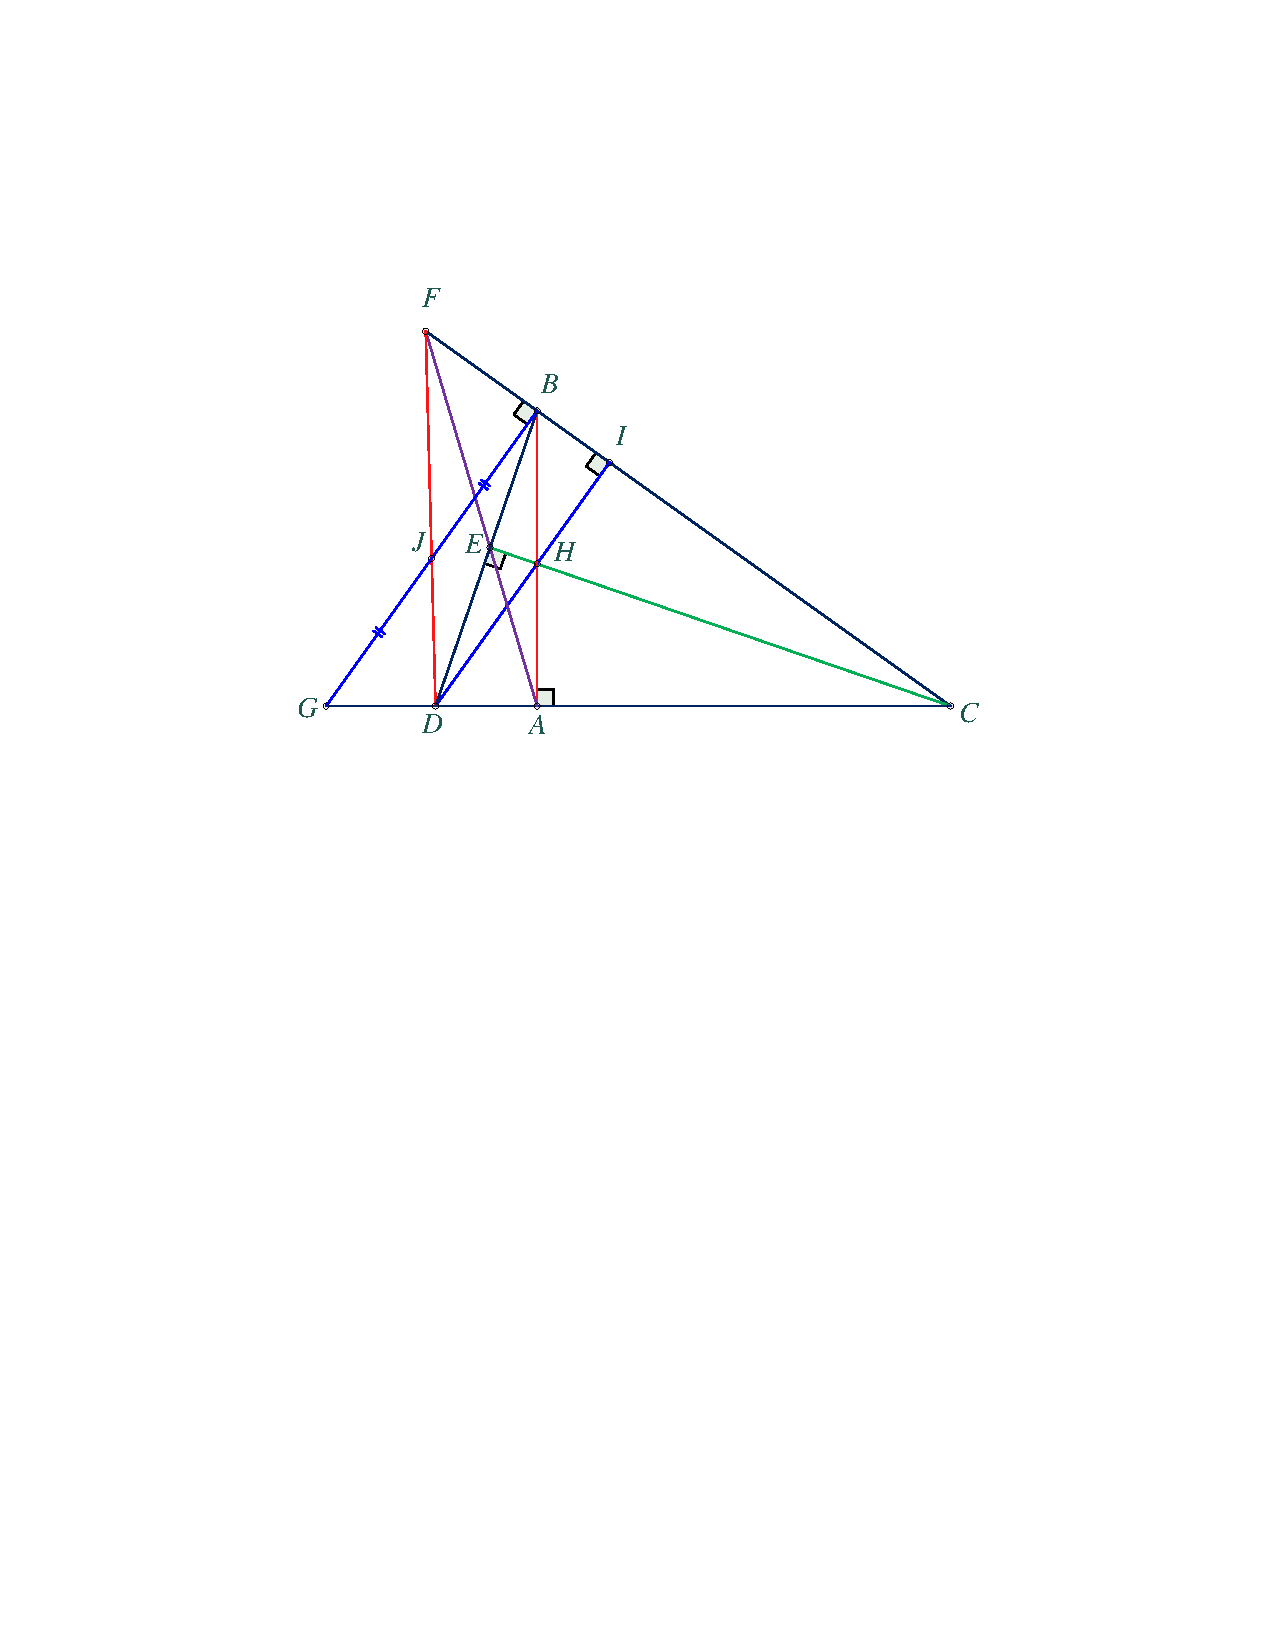
\includegraphics[width=0.9\linewidth]{P615H1}
		\vspace*{-15pt}
	\end{figure}
	Gọi $J$ là giao điểm của $GB$ và $DF$; do $D \not\equiv G$  và $F \not\equiv B$,  nên $J$ nằm giữa $D$ và $F$.
	\vskip 0.05cm
	Gọi $H$ là giao điểm của $CE$ và $AB$; $I$ là giao điểm của $DH$ và $BC$.
	\vskip 0.05cm
	Do $BA \bot CD$ và $CE \bot BD$, nên $H$ là trực tâm tam giác $BCD$; suy ra, $DI \bot BC$. \hfill                                   ($1$)
	\vskip 0.05cm
	Áp dụng định lý Ceva cho tam giác $BCD$, với ba đường đồng quy $BA$, $CE$, $DI$, ta được:
	\begin{align*}
		\frac{{IC}}{{IB}} \cdot \frac{{EB}}{{ED}} \cdot \frac{{AD}}{{AC}} = 1. \tag{$2$}
	\end{align*}
	Từ ($1$) và định nghĩa điểm $G$, suy ra $DI \parallel GB$. Do đó, theo định lý Thales, ta có:
	\begin{align*}
		\frac{{DC}}{{DG}} = \frac{{IC}}{{IB}} \cdot \tag{$3$}
	\end{align*}
	Áp dụng định lý Menelaus lần lượt cho tam giác $BCD$, với cát tuyến $AEF$, và cho tam giác $BCG$, với cát tuyến $DJF$, ta được:
	\begin{align*}
		&\frac{{FB}}{{FC}} \cdot \frac{{AC}}{{AD}} \cdot \frac{{ED}}{{EB}} = 1. \tag{$4$}\\
		&\frac{{JB}}{{JG}} \cdot \frac{{DG}}{{DC}} \cdot \frac{{FC}}{{FB}} = 1.\tag{$5$}
	\end{align*}
	Từ ($4$) suy ra
	\begin{align*}
		\frac{{FB}}{{FC}} = \frac{{AD}}{{AC}} \cdot \frac{{EB}}{{ED}} \cdot \tag{$6$}
	\end{align*}
	Từ ($5$), ($3$), ($6$) và ($2$), suy ra
	\begin{align*}
		\frac{{JB}}{{JG}} = \frac{{DC}}{{DG}} \cdot \frac{{FB}}{{FC}} = \frac{{IC}}{{IB}} \cdot \frac{{EB}}{{ED}} \cdot \frac{{AD}}{{AC}} = 1;
	\end{align*}
	do đó, $J$ là trung điểm của $BG$. Mà $B$, $G$ cố định nên $J$ là một điểm cố định.
	\vskip 0.05cm
	Như vậy, trong trường hợp này, $DF$ luôn đi qua điểm cố định $J$.
	\vskip 0.05cm
	$\bullet$ \textit{Trường hợp} $3$: $BD \bot BC$.
	\vskip 0.05cm
	Khi đó, $D \equiv G$; suy ra, $E \equiv B \equiv F$. Vì thế, đường thẳng $DF$ cũng chính là đường thẳng $BG$; do đó, $DF$ đi qua điểm cố định $J$.
	\begin{figure}[H]
		\centering
		\vspace*{-5pt}
		\captionsetup{labelformat= empty, justification=centering}
		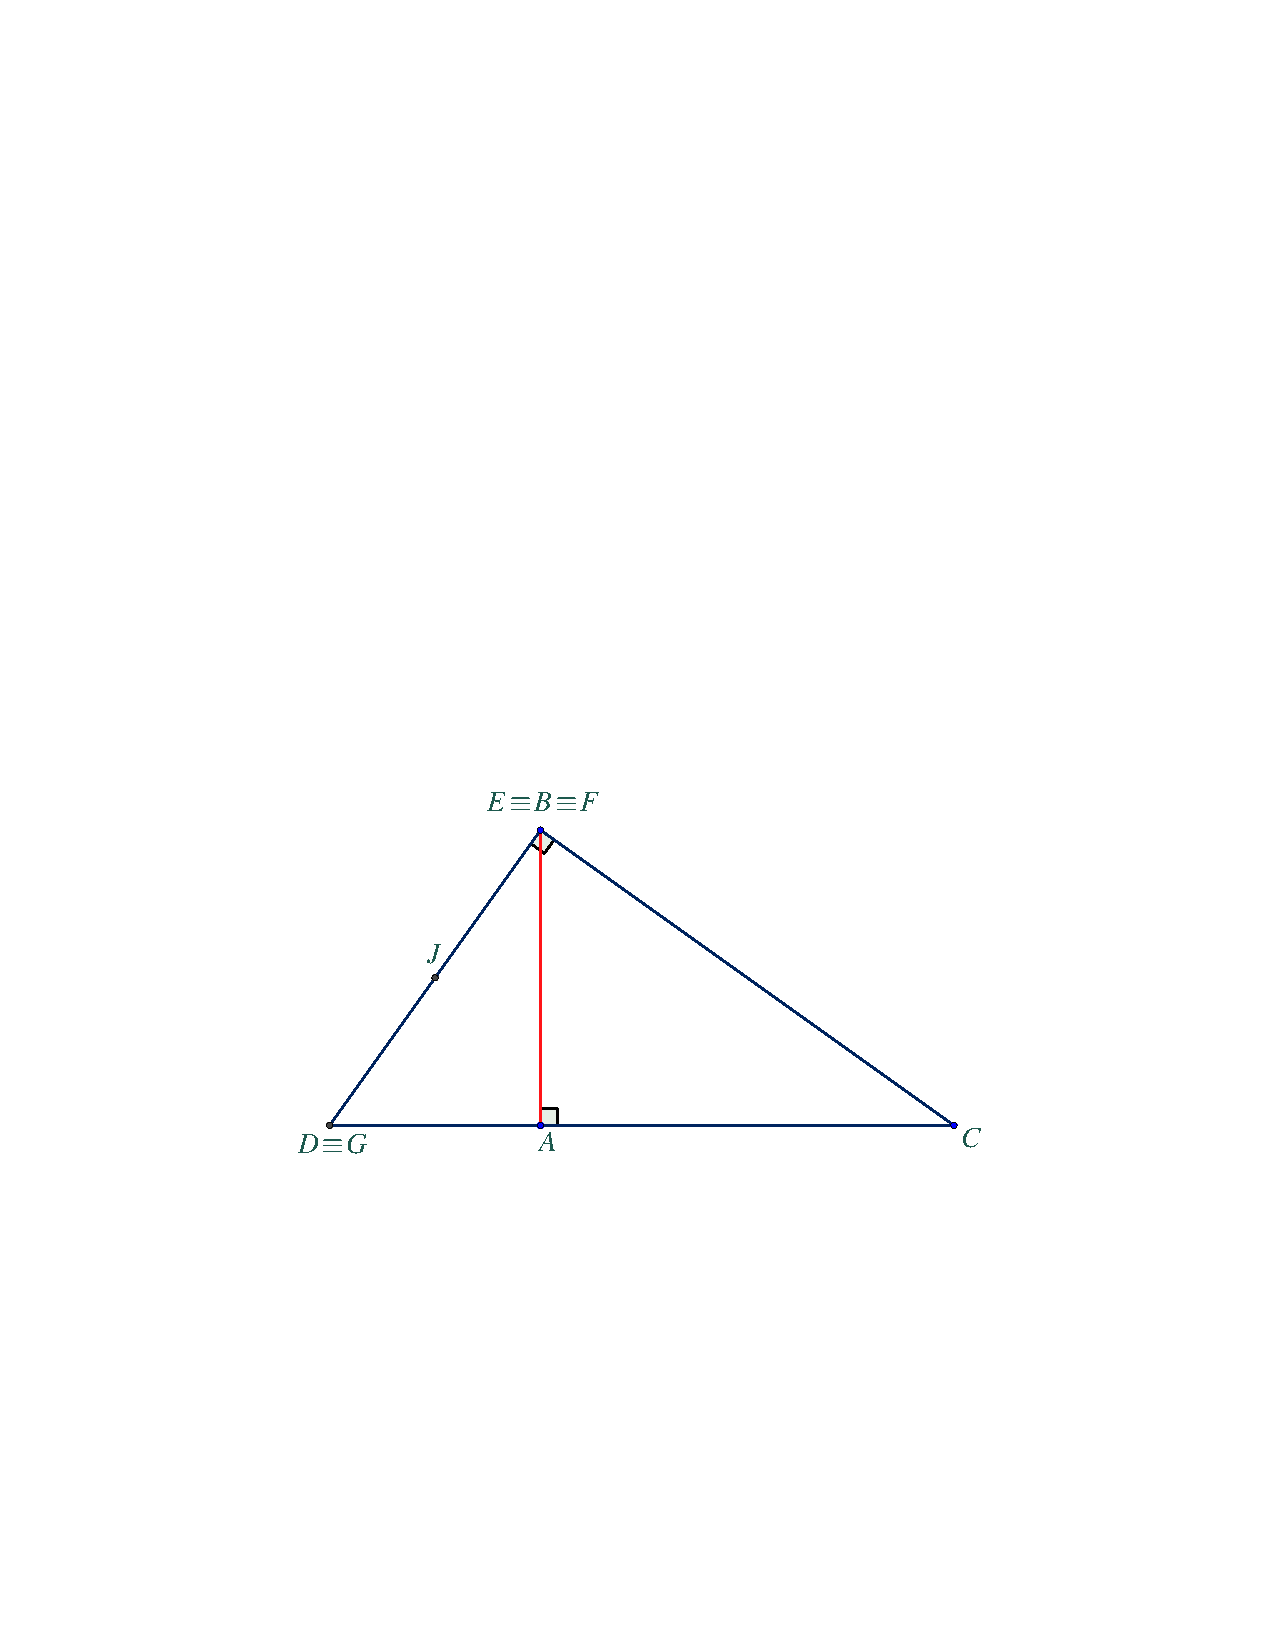
\includegraphics[width=0.9\linewidth]{P615H2}
		\vspace*{-15pt}
	\end{figure}
	$\bullet$ \textit{Trường hợp} $4$: $D \equiv C$.
	\vskip 0.05cm
	Khi đó, $E \equiv C$, và do đó, $F \equiv C$. Vì thế, bất kỳ đường thẳng nào đi qua $C$ cũng có thể được coi là đường thẳng $DF$. Do vậy, coi đường thẳng $CJ$ là đường thẳng $DF$, ta sẽ có $DF$ đi qua điểm cố định $J$.
	\vskip 0.05cm
	Vậy, tóm lại, khi điểm $D$ di động trên tia $CA$, sao cho  $D \not\equiv A$ đường thẳng $DF$ luôn đi qua điểm cố định $J$, là trung điểm của đoạn thẳng $BG$, với $G$ là điểm nằm trên tia $CA$, thỏa mãn $GB \bot BC$.
	\vskip 0.05cm
	\textbf{\color{thachthuctoanhoc}Bình luận và Nhận xét}
	\vskip 0.05cm
	Do không xét các trường hợp $3$, $4$, được nêu ở lời giải trên, nên ở tất cả các lời giải Tạp chí nhận được từ bạn đọc đều có những tỷ số có mẫu \textit{không} luôn khác $0$. Vì thế, tất cả lời giải Tạp chí nhận được từ bạn đọc đều là lời giải không chính xác.
	\begin{flushright}
		\textbf{\color{thachthuctoanhoc}Hạ Vũ Anh}
	\end{flushright}
	{\color{thachthuctoanhoc}{\usefont{T5}{qag}{b}{n} P616.}}
	(Mức $B$) Xét các số dương $a,b,c$ thoả mãn $a+b+c=4$. Tìm giá trị nhỏ nhất của biểu thức 
	\begin{align*}
		P=\left|\dfrac 1a-1\right|+\left|\dfrac 1b-1\right|+\left|\dfrac 1c-1\right|.
	\end{align*}
	\textbf{\color{thachthuctoanhoc}Lời giải} (\textit{dựa theo lời giải của bạn Trần Việt Anh, lớp $8$C$1$, trường TH, THCS $\color{black}\&$ THPT Archimedes, Đông Anh, Tp. Hà Nội})\textbf{\color{thachthuctoanhoc}.}
	\vskip 0.05cm
	Do $a$, $b$, $c$ có vai trò như nhau trong biểu thức $P$ nên không mất tính tổng quát, có thể giả sử $a = \max\{a, b, c\}$.
	\vskip 0.05cm
	Xét hai trường hợp sau:
	\vskip 0.05cm
	$\bullet$ \textit{Trường hợp} $1$: $a > 2$.
	\vskip 0.05cm
	Khi đó, $\dfrac{1}{a} < \dfrac{1}{2}$  suy ra
	\begin{align*}
		\frac{1}{a} - 1 < \frac{1}{2} - 1 =  - \frac{1}{2}.
	\end{align*}
	Do đó
	\begin{align*}
		\left| {\frac{1}{a} - 1} \right| > \left| { - \frac{1}{2}} \right| = \frac{1}{2}.
	\end{align*}
	Vì thế
	\begin{align*}
		P \ge \left| {\frac{1}{a} - 1} \right| > \frac{1}{2}.
	\end{align*}
	$\bullet$ \textit{Trường hợp} $2$: $0 < a \le 2$.
	\vskip 0.05cm
	Khi đó, $\dfrac{1}{a} \ge \dfrac{1}{2}$; do đó, với lưu ý tới các giả thiết của bài ra, ta có:
	\begin{align*}
			P &= \frac{{\left| {a - 1} \right|}}{a} + \frac{{\left| {b - 1} \right|}}{b} + \frac{{\left| {c - 1} \right|}}{c} \\
			&\ge \frac{{\left| {a - 1} \right|}}{a} + \frac{{\left| {b - 1} \right|}}{a} + \frac{{\left| {c - 1} \right|}}{a}\\
			&\quad({\text{\color{black} do } } a = \max \{ a,b,c\} )\\
			 &= \frac{{\left| {a - 1} \right| + \left| {b - 1} \right| + \left| {c - 1} \right|}}{a} \\
			 &\ge \frac{{\left| {a + b + c - 3} \right|}}{a} = \frac{1}{a} \ge \frac{1}{2}.
	\end{align*}
	Như vậy, với mọi số thực dương $a$, $b$, $c$, thỏa mãn điều kiện của đề bài, ta luôn có  $P \ge \dfrac{1}{2}$.
	\vskip 0.05cm
	Hơn nữa, với $a \!=\! 2$, $b \!=\! c \!=\! 1$, ta có $a, b, c \!>\! 0$, $a + b + c = 4$, và  $P = \dfrac{1}{2}$.
	\vskip 0.05cm
	Vì vậy, giá trị nhỏ nhất của $P$ bằng  $\dfrac{1}{2}$.
	\vskip 0.05cm
	\textbf{\color{thachthuctoanhoc}Bình luận và Nhận xét}
	\vskip 0.05cm
	$\pmb{1.}$ Ở lời giải trên, ta đã sử dụng (không chứng minh) bất đẳng thức ``trị tuyệt đối" rất cơ bản sau:
	\vskip 0.05cm
	``\textit{Cho số nguyên $n \ge 2$. Khi đó, với mọi  $x_1, x_2, \ldots,x_n \in \mathbb{R}$, ta có:}
	\begin{align*}
		|{x_1}| \!+\! |{x_2}| \!+\!  \cdots  \!+\! |{x_n}| \!\ge\! |{x_1} \!+\! {x_2} \!+\!  \cdots  \!+\! {x_n}|. \text{\color{black}"}
	\end{align*}
	Bạn đọc có thể dễ dàng chứng minh bất đẳng thức trên bằng phương pháp quy nạp theo $n \ge 2$.
	\vskip 0.05cm
	$\pmb{2.}$ Rất tiếc, có tới một nửa số lời giải Tạp chí nhận được từ bạn đọc là lời giải sai, hoặc không hoàn chỉnh, do người giải bài đã mắc một trong các lỗi sau:
	\vskip 0.05cm
	$\diamond$ Ngộ nhận rằng, với  $x,y \in \mathbb{R}$ nếu $x \ge y$ thì $|x|\ge |y|$.
	\vskip 0.05cm 
	$\diamond$ Khẳng định giá trị nhỏ nhất của $P$ bằng  $\dfrac{1}{2}$, ngay sau khi mới chỉ chứng minh được  $P \ge \dfrac{1}{2}$.
	\vskip 0.05cm
	\hfill	\textbf{\color{thachthuctoanhoc}Nguyễn Khắc Minh}
	\vskip 0.05cm
	{\color{thachthuctoanhoc}{\usefont{T5}{qag}{b}{n} P617.}}
	(Mức $A$) Giải phương trình
	\begin{align*}
		\sqrt{(x^3-4)^3}=\sqrt[3]{(x^2+4)^2}+4.
	\end{align*} 
	\textbf{\color{thachthuctoanhoc}Lời giải} (\textit{dựa theo lời giải của bạn Trần Hữu Dương, lớp $10$ Toán $1$, trường THPT chuyên Hưng Yên, tỉnh Hưng Yên})\textbf{\color{thachthuctoanhoc}.}
	\vskip 0.05cm
	Điều kiện xác định của phương trình:\linebreak $x \ge \sqrt[3]{4}$. \hfill ($1$)
	\vskip 0.05cm
	Đặt $\sqrt {{x^3} - 4}  = a$,   $\sqrt[3]{{{x^2} + 4}} = b$; khi đó, phương trình đã cho được viết lại dưới dạng:
	\begin{align*}
		{a^3} = {b^2} + 4. \tag{$2$}
	\end{align*}
	Từ định nghĩa của $a$, $b$, ta có:
	\begin{align*}
		&{a^2} - {b^3} = {x^3} - {x^2} - 8, \tag{$3$}\\
		&{a^2} - {x^2} = {x^3} - {b^3} = {x^3} - {x^2} - 4.\tag{$4$}
	\end{align*}
	Từ ($2$) và ($3$), suy ra
	\begin{align*}
		{a^3} - {x^3} + {x^2} - {b^2} + {a^2} - {b^3} + 4 = 0. \tag{$5$}
	\end{align*}
	Do ($1$), và do $a \ge 0$, $b > 0$, nên $a + x > 0$, $x + b > 0$, và
	\begin{align*}
		{x^2} + ax + {a^2} > 0,\,\,\, {x^2} + bx + {b^2} > 0.
	\end{align*}
	Vì thế, với lưu ý tới ($3$), ($4$), ta có:
	\begin{align*}
		&(5) \\[-0.5ex]
		\Leftrightarrow &\left( {a - x} \right)\left( {{a^2} + ax + {x^2}} \right) + \left( {x - b} \right)\left( {x + b} \right) \\[-0.5ex]
		&+ \left( {{x^3} - {x^2} - 4} \right) = 0\\[-0.5ex]
		\Leftrightarrow &\frac{{\left( {{a^2} \!-\! {x^2}} \right)\!\!\left( {{a^2} \!+\! ax \!+\! {x^2}} \right)}}{{a \!+\! x}} \!+\! \frac{{\left( {{x^3} \!-\! {b^3}} \right)\!\!\left( {x \!+\! b} \right)}}{{{x^2} \!+\! bx \!+\! {b^2}}} \\[-0.5ex]
		&+ \left( {{x^3} - {x^2} - 4} \right) = 0\\[-0.5ex]
		\Leftrightarrow &\left( {{x^3} - {x^2} - 4} \right)\\
		&\times\!\!\left(\!\! {\frac{{{a^2} \!+\! ax \!+\! {x^2}}}{{a + x}} \!+\! \frac{{x + b}}{{{x^2} + bx + {b^2}}} \!+\! 1} \right) \!=\! 0\\[-0.5ex]
		\Leftrightarrow &\,\,{x^3} \!-\! {x^2} \!-\! 4 \!=\! 0 \Leftrightarrow  \left( {x \!-\! 2} \right)\!\!\left( {{x^2} \!+\! x \!+\! 2} \right) \!=\! 0\\[-0.5ex]
		\Leftrightarrow &\,\,x = 2 \quad(\text{\color{black}do } x^2 + x + 2 > 0).
	\end{align*}
	Bằng cách thử trực tiếp, ta thấy $x = 2$ nghiệm đúng phương trình đã cho.
	\vskip 0.05cm
	Vậy, phương trình đã cho có nghiệm duy nhất $x = 2$.
	\vskip 0.05cm
	\textbf{\color{thachthuctoanhoc}Bình luận và Nhận xét}
	\vskip 0.05cm
	$\pmb{1.}$ Ở lời giải trên, phép thử lại là bắt buộc, do phép biến đổi từ ($2$) sang ($5$) là phép biến đổi hệ quả.
	\vskip 0.05cm
	$\pmb{2.}$ Tất cả lời giải Tạp chí nhận được từ bạn đọc đều có cách giải đúng và đáp số đúng. Tuy nhiên, một số lời giải trong số đó \textit{không} được coi là lời giải hoàn chỉnh, do người giải bài quên (?) không tìm điều kiện xác định của phương trình đã cho, trước khi tiến hành các biến đổi.
	\vskip 0.05cm
	\hfill	\textbf{\color{thachthuctoanhoc}Nguyễn Khắc Minh}
	\vskip 0.05cm
	{\color{thachthuctoanhoc}{\usefont{T5}{qag}{b}{n} P618.}}
	(Mức $A$) Cho $a,b,c$ là các số nguyên lớn hơn $1$. Giả sử $x,y,z$ là các số thực thoả mãn $a^x=bc$, $b^y=ca$ và $c^z=ab$. Tính giá trị của biểu thức $T=x+y+z-xyz$. 
	\vskip 0.05cm
	\textbf{\color{thachthuctoanhoc}Lời giải} (\textit{dựa theo lời giải của các bạn: Nguyễn Đức Khải, Trần Đình Nam (lớp $10$T$2$, trường THPT chuyên Lê Hồng Phong, tỉnh Nam Định) và Nguyễn Đình Khải Nguyên, Trần Thị Thanh Thư (lớp $11$T$2$, $12$T$1$, trường THPT chuyên Quốc học Huế, tỉnh Thừa Thiên -- Huế)}).
	\vskip 0.05cm
	Từ các giả thiết của bài ra, ta có:
	\begin{align*}
		{a^{xyz}} &= {\left( {bc} \right)^{yz}} = {\left( {{b^y}} \right)^z} \cdot {\left( {{c^z}} \right)^y} = {\left( {ca} \right)^z} \cdot {\left( {ab} \right)^y} \\[-0.5ex]
		&= {a^{y + z}} \cdot {c^z} \cdot {b^y} = {a^{y + z}} \cdot \left( {ab} \right)\left( {ca} \right) \\[-0.5ex]
		&= {a^{y + z + 2}} \cdot \left( {bc} \right) = {a^{x + y + z + 2}}.
	\end{align*}
	Từ đó, do $a \ne 1$, suy ra
	\begin{align*}
		xyz = x + y + z + 2.
	\end{align*}
	Vì thế
	\begin{align*}
		T = x + y + z - xyz = -2.
	\end{align*}
	\textbf{\color{thachthuctoanhoc}Bình luận và Nhận xét}
	\vskip 0.05cm
	Tất cả các lời giải Tạp chí nhận được từ bạn đọc đều là lời giải đúng.
	\vskip 0.05cm
	\hfill	\textbf{\color{thachthuctoanhoc}Lê Huy}
	\vskip 0.05cm
	{\color{thachthuctoanhoc}{\usefont{T5}{qag}{b}{n} P619.}}
	(Mức $A$) Cho tam giác $ABC$ nội tiếp đường tròn $(O)$, có trực tâm $H$. Gọi $M$ là điểm chính giữa cung $BAC$ của $(O)$. Qua $O$ kẻ đường thẳng  song song với $AM$, cắt $HM$ tại $P$. Gọi $X,Y,Z$ tương ứng là hình chiếu vuông góc của $P$ trên $BC,CA,AB$. Chứng minh rằng, đường tròn ngoại tiếp tam giác $XYZ$ đi qua trung điểm của $HM.$
	\vskip 0.05cm
	\textbf{\color{thachthuctoanhoc}Lời giải} (\textit{dựa theo Đáp án do Ban biên tập Tạp chí cung cấp})\textbf{\color{thachthuctoanhoc}.}
	\vskip 0.05cm
	Dễ thấy, khi $ABC$ là tam giác vuông tại $A$ thì điểm $P$ không tồn tại (do khi đó, hai đường thẳng $AM$ và $HM$ trùng nhau). \textit{Dưới đây là lời giải cho bài đã ra, với giả thiết tam giác $ABC$ không vuông tại $A$}.
	\vskip 0.05cm
	Gọi $N$ là điểm chính giữa cung $BC$ không chứa $A$ của $(O)$; gọi $D$ là trung điểm của $BC$; và gọi $T$ là giao điểm của tiếp tuyến tại $B$ và tiếp tuyến tại $C$ của $(O)$. Ta có, năm điểm $M$, $O$, $D$, $N$, $T$ cùng nằm trên đường trung trực của $BC$, và $N$ là trung điểm của $OT$. (Xem Hình $1$.)
	\begin{figure}[H]
		\centering
		\vspace*{-10pt}
		\captionsetup{labelformat= empty, justification=centering}
		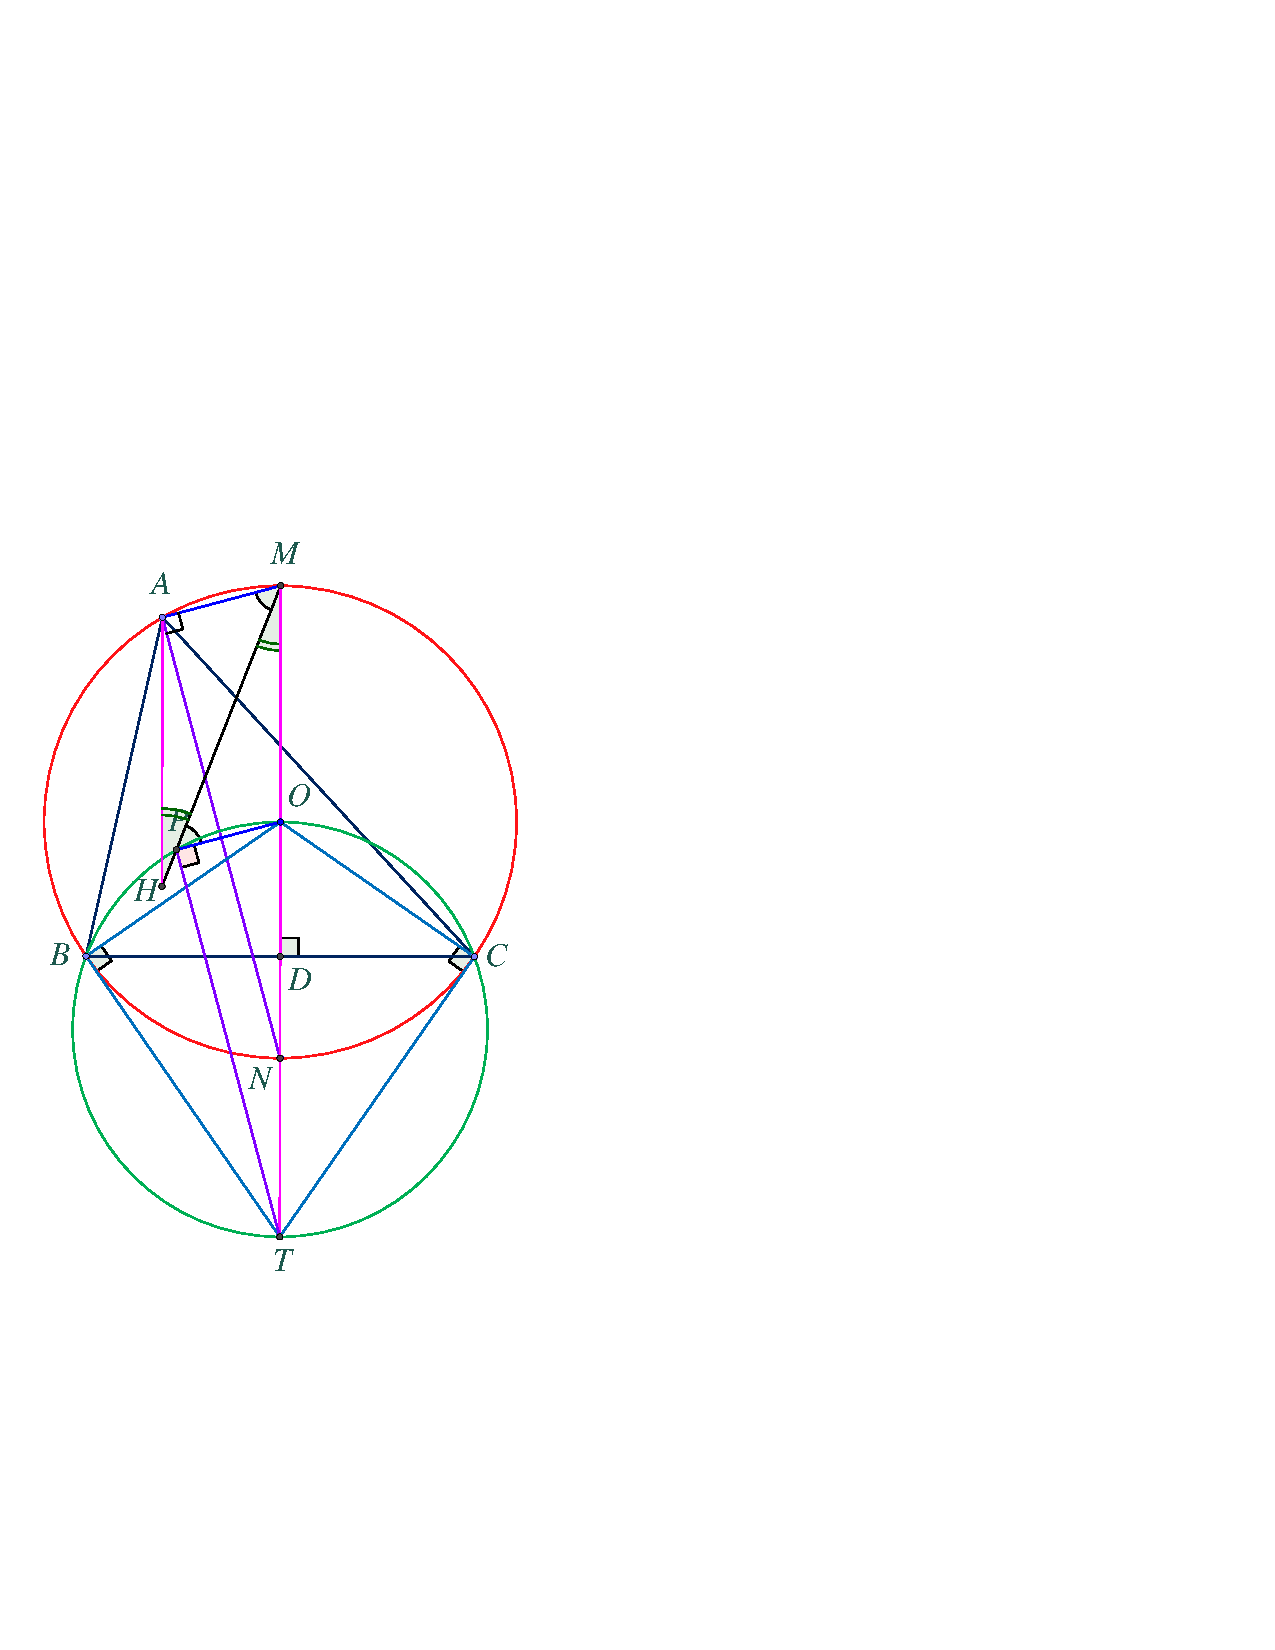
\includegraphics[width=0.68\linewidth]{P619H1}
		\caption{\small\textit{\color{thachthuctoanhoc}Hình $1$.}}
		\vspace*{-10pt}
	\end{figure}
	Vì $D$ là trung điểm $BC$, và $H$, $O$ tương ứng là trực tâm, tâm đường tròn ngoại tiếp tam giác $ABC$, nên $AH = 2OD$. \hfill ($1$)
	\vskip 0.05cm
	Vì $AH \parallel MO$ (do cùng vuông góc với $BC$) và $AM \parallel PO$ (theo giả thiết), nên
	\begin{align*}
		\angle MHA = \angle PMP \text{\color{black}\, và } \angle HMA = \angle MPO.
	\end{align*}
	Do đó, $\Delta AMH \sim \Delta OPM$. Kết hợp với ($1$), suy ra
	\begin{align*}
		\frac{{AM}}{{OP}} = \frac{{HA}}{{MO}} = \frac{{2OD}}{{MO}} \cdot \tag{$2$}
	\end{align*}
	Vì $CT$ là tiếp tuyến tại $C$ của $(O)$ nên $OCT$ là tam giác vuông tại $C$. Do đó
	\begin{align*}
		O{C^2} = OD \cdot OT;
	\end{align*}
	suy ra
	\begin{align*}
		\frac{{OD}}{{MO}} = \frac{{OD}}{{OC}} = \frac{{OC}}{{OT}} \cdot
	\end{align*}
	Vì thế
	\begin{align*}
		\frac{{2OD}}{{MO}} = \frac{{2OC}}{{OT}} = \frac{{MN}}{{OT}} \cdot \tag{$3$}
	\end{align*}
	Từ ($2$) và ($3$), suy ra
	\begin{align*}
		\frac{{AM}}{{PO}} = \frac{{MN}}{{OT}} \cdot \tag{$4$}
	\end{align*}
	Vì $AM \parallel PO$ (theo giả thiết), nên \linebreak$\angle AMN = \angle POT$.  Kết hợp với ($4$), suy ra $\Delta AMN \sim  \Delta POT$. Do đó
	\begin{align*}
		\angle OPT = \angle MAN = 90^\circ. \tag{$5$}
	\end{align*}
	Vì vậy, $P$ nằm trên đường tròn đường kính $OT$. Mà đường tròn này chính là đường tròn ngoại tiếp tam giác $OBC$ (do các tam giác $OBT$, $OCT$, tương ứng, vuông góc tại $B$, $C$, và $N$ là trung điểm của $OT$), nên ta có năm điểm $P$, $O$, $B$, $T$, $C$ cùng nằm trên đường tròn đường kính $OT$. \hfill                                            ($6$)
	\vskip 0.05cm
	Gọi $E$, $F$ tương ứng là giao điểm của $PT$ và $AB$, $AC$; gọi $Q$ là trung điểm của $HM$. (Xem Hình $2$.)
	\begin{figure}[H]
		\centering
		\vspace*{-10pt}
		\captionsetup{labelformat= empty, justification=centering}
		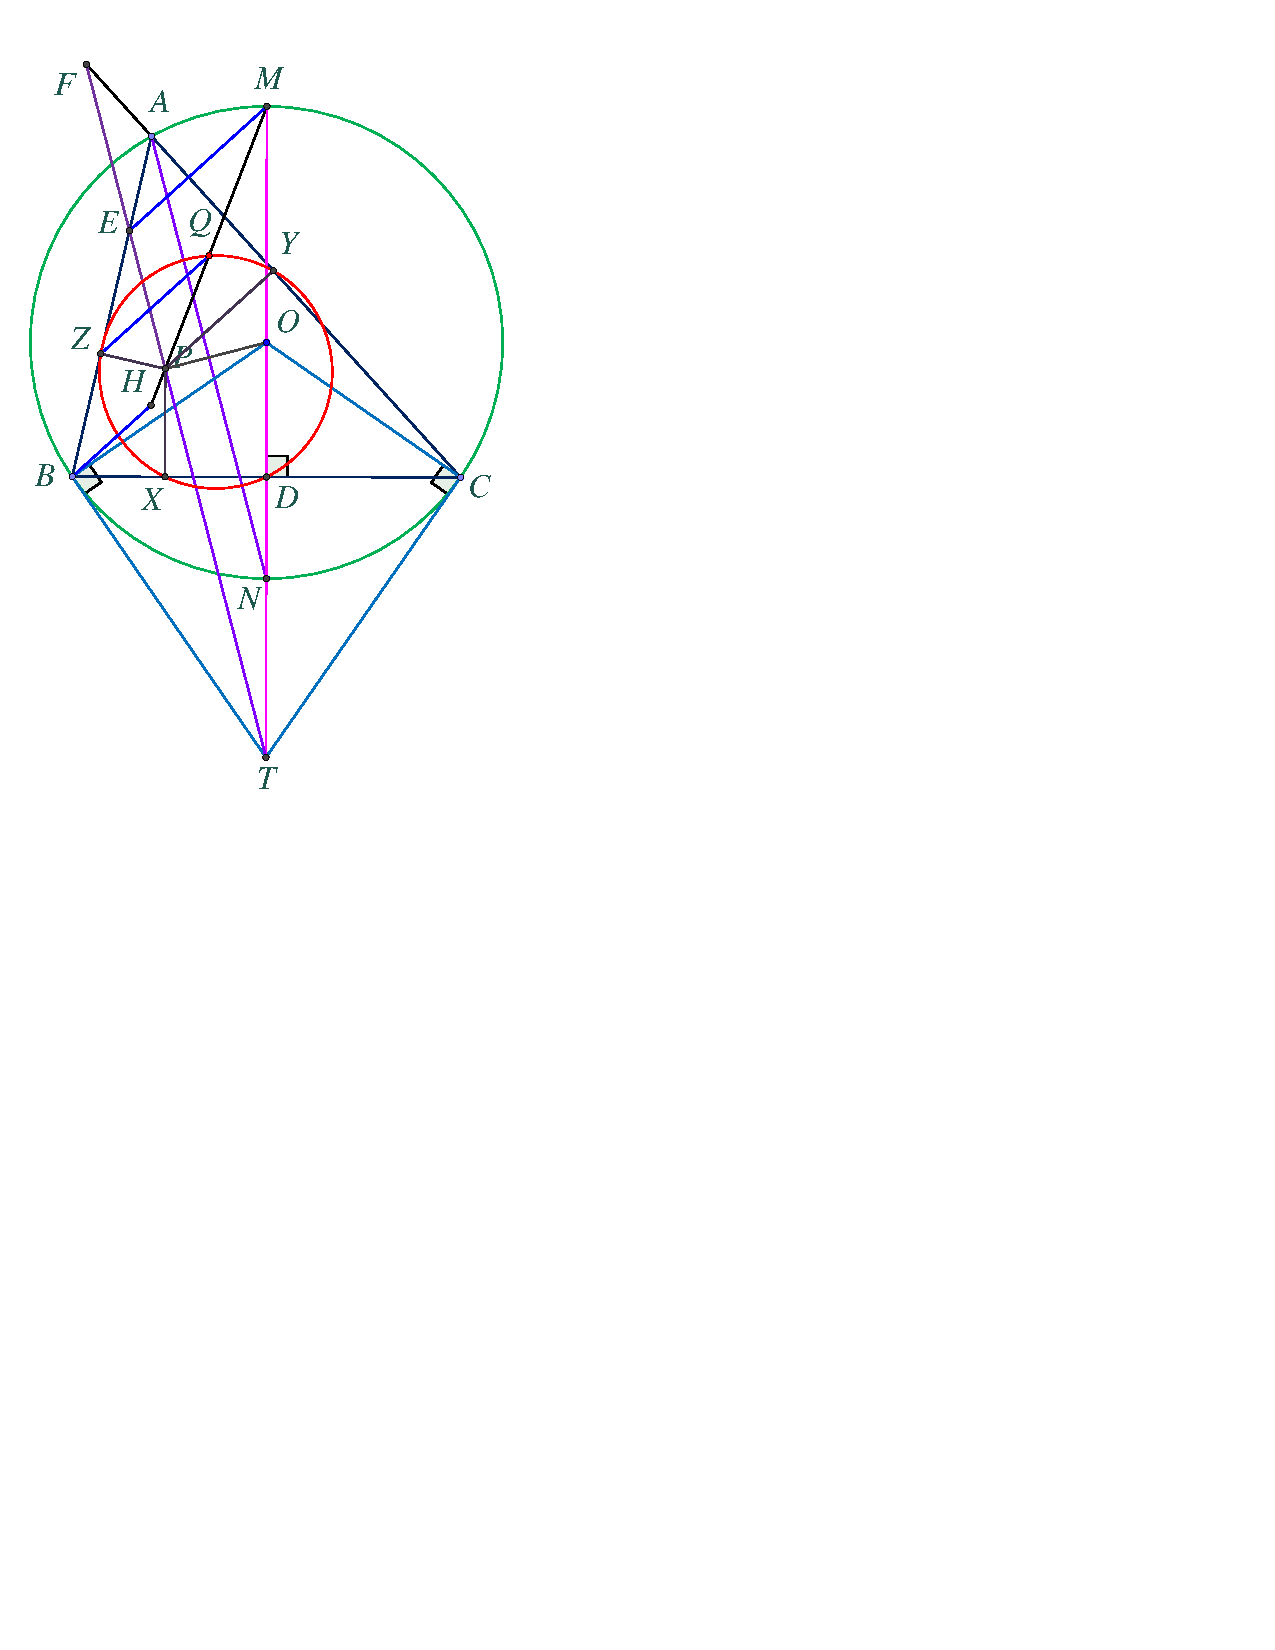
\includegraphics[width=0.7\linewidth]{P619H2}
		\caption{\small\textit{\color{thachthuctoanhoc}Hình $2$.}}
		\vspace*{-5pt}
	\end{figure}
	Từ ($5$) và giả thiết $AM \parallel PO$, suy ra:
	\begin{align*}
		AN \parallel PT. \tag{$7$}
	\end{align*}
	Do đó
	\begin{align*}
		\angle BEP &= \angle BET = \angle BAN = \angle BMN \\
		&= \frac{1}{2}\angle BMC = \frac{1}{2}\angle BCT \\
		&= \frac{1}{2}\angle BPT\,\,({\text{\color{black}do }}(6)).
	\end{align*}
	Suy ra, tam giác $BEP$ cân tại $P$; vì thế, $Z$ là trung điểm của $BE$. \hfill ($8$)
	\vskip 0.05cm
	Lại do ($7$) nên
	\begin{align*}
		\angle MTE = \angle MNA = \angle MBA = \angle MBE;
	\end{align*}
	suy ra, $BEMT$ là tứ giác nội tiếp. Do đó
	\begin{align*}
			\angle AEM &= \angle BTM = \angle BTO \\
			&= \angle BCO \,\,({\text{\color{black}do }}(6))\\
			 &= 90^\circ - \frac{1}{2}\angle BOC = 90^\circ - \angle BAC;
	\end{align*}
	suy ra, $EM \bot AC$. Vì thế, $EM \parallel BH$. Do vậy, tứ giác $BHME$ là một hình thang. Vì thế, từ định nghĩa điểm $Q$ và ($8$), suy ra $ZQ \parallel BH$. Do đó, $ZQ \bot AY$. \hfill ($9$)
	\vskip 0.05cm
	Bằng cách hoàn toàn tương tự, ta cũng chứng minh được $Y$ là trung điểm của $CF$, $CMFT$ là tứ giác nội tiếp, và $YQ \bot AZ$. \hfill ($10$)
	\vskip 0.05cm
	Từ ($9$) và ($10$) suy ra, $Q$ là trực tâm tam giác $AZY$. Do đó
	\begin{align*}
		\angle ZQY &= 180^\circ - \angle ZAY \\
		&= 180^\circ - \angle BAC. \tag{$11$}
	\end{align*}
	Do $BXPZ$, $CXPY$, $BEMT$, $CMFT$ là các tứ giác nội tiếp, nên
	\begin{align*}
			\angle ZXY &= \!\angle ZXP \!+\! \angle PXY \!=\! \angle ZBP \!+\! \angle PCY\\
			&= \angle ZEP + \angle PFY \,\,({\text{\color{black}do }}(8) \,\,\text{\color{black}và }(10))\\
			&= \!\angle BET \!\!+\!\! \angle TFC \!\!=\!\! \angle BMT \!\!+\!\! \angle TMC\\
			&= \angle BMC = \angle BAC.\tag{$12$}
	\end{align*}
	Từ ($11$) và ($12$), suy ra
	\begin{align*}
		\angle ZQY + \angle ZXY = 180^\circ;
	\end{align*}
	do đó, $ZQYX$ là tứ giác nội tiếp.
	\vskip 0.05cm
	Ta có điều phải chứng minh theo yêu cầu đề bài.
	\vskip 0.05cm
	\textbf{\color{thachthuctoanhoc}Bình luận và Nhận xét}
	\vskip 0.05cm
	Tất cả các lời giải Tạp chí nhận được từ bạn đọc đều là lời giải đúng, cho bài đã ra với giả thiết tam giác $ABC$ không vuông tại $A$.
	\begin{flushright}
		\textbf{\color{thachthuctoanhoc}Hạ Vũ Anh}
	\end{flushright}
	{\color{thachthuctoanhoc}{\usefont{T5}{qag}{b}{n} P620.}}
	(Mức $A$) Chứng minh rằng với mọi số nguyên tố $p\ge5$, tồn tại số nguyên $t$ sao cho: với mọi số nguyên $k$ thì $k^2-2t^2-1$ không chia hết cho $p$.   
	\vskip 0.05cm
	\textbf{\color{thachthuctoanhoc}Lời giải} (\textit{của người chấm bài})\textbf{\color{thachthuctoanhoc}.}
	\vskip 0.05cm
	Nhắc lại định nghĩa \textit{ký hiệu Legendre}: Với $a$ là số nguyên, và $p$ là số nguyên tố, ký hiệu:
	\begin{align*}
		\hspace*{-6pt}\left(\!\!\frac{a}{p}\!\right) \!\!= \!\!\begin{cases}
			0 \text{ nếu } p \mid a\\
			1 \text{ nếu } p\nmid a \text{ và } \exists\, x \!\in\! \mathbb{Z}:\! x^2 \!\equiv\! a (\!\!\bmod p)\\
			\!\!\!\!\!-\!1 \text{ nếu } p\nmid a \text{ và } \overline{\exists}\, x \!\in\! \mathbb{Z}:\! x^2 \!\equiv\! a (\!\!\bmod p).
		\end{cases}
	\end{align*}
	Trước hết, ta chứng minh hai Bổ đề sau:
	\vskip 0.05cm
	\textbf{\color{thachthuctoanhoc}Bổ đề} $\pmb{1.}$ Với $p$ là một số nguyên tố lẻ, và $k$ là một số nguyên dương nhỏ hơn $p - 1$, ta có:
	\begin{align*}
		{1^k} + {2^k} +  \cdots  + {\left( {p - 1} \right)^k} \equiv 0\left( {\bmod p} \right).
	\end{align*}
	\textit{Chứng minh}. Đặt $S = {1^k} + {2^k} +  \cdots  + {\left( {p - 1} \right)^k}$.
	\vskip 0.05cm   
	Do $k < p - 1$ nên theo định lý Lagrange, phương trình
	\begin{align*}
		{x^k} - 1 \equiv 0\left( {\bmod p} \right)
	\end{align*}
	có tối đa $k$ nghiệm modulo $p$. Vì vậy, tồn tại $a \in \{1; 2; \ldots; p - 1\}$ sao cho
	\begin{align*}
		{a^k}\not  \equiv 1\left( {\bmod p} \right). \tag{$1$}
	\end{align*}
	Do $\{a, 2a, \ldots, (p - 1)a\}$ là một hệ thặng dư thu gọn modulo $p$, nên
	\begin{align*}
		S &\equiv {a^k} + {\left( {2a} \right)^k} +  \cdots  + {\left( {\left( {p - 1} \right)a} \right)^k} \\
		&= {a^k} \cdot S\left( {\bmod p} \right). \tag{$2$}
	\end{align*}
	Từ ($1$) và ($2$), suy ra $S \equiv 0\left( {\bmod p} \right)$.
	\vskip 0.05cm 
	Bổ đề $1$ được chứng minh.
	\vskip 0.05cm
	\textbf{\color{thachthuctoanhoc}Bổ đề} $\pmb{2.}$ Nếu $p$ là một số nguyên tố lẻ thì
	\begin{align*}
		\sum\limits_{i = 0}^{p - 1} {\left( {\frac{{2{i^2} + 1}}{p}} \right)}  \equiv  \pm 1\left( {\bmod p} \right).
	\end{align*}
	\textit{Chứng minh}. Theo tiêu chuẩn Euler, ta có:
	\begin{align*}
		&\sum\limits_{i = 0}^{p - 1} {\left( {\frac{{2{i^2} + 1}}{p}} \right)} \\ \equiv &\sum\limits_{i = 0}^{p - 1} {{{\left( {2{i^2} + 1} \right)}^{\frac{{p - 1}}{2}}}} \left( {\bmod p} \right). \tag{$3$}	
	\end{align*}
	Do
	\begin{align*}
		&\sum\limits_{i = 0}^{p - 1} {{{\left( {2{i^2} + 1} \right)}^{\frac{{p - 1}}{2}}}}  \\
		= &\sum\limits_{i = 0}^{p - 1} {\sum\limits_{s = 0}^{\left( {p - 1} \right)/2} {{\rm{C}}_{\left( {p - 1} \right)/2}^s{{\left( {2{i^2}} \right)}^s}} }  \\
		= &\sum\limits_{s = 0}^{\left( {p - 1} \right)/2} {{2^s}{\rm{C}}_{\left( {p - 1} \right)/2}^s\sum\limits_{i = 0}^{p - 1} {{i^{2{\rm{s}}}}} }
	\end{align*}
	nên theo ($3$), ta có:
	\begin{align*}
		&\sum\limits_{i = 0}^{p - 1} {\left( {\frac{{2{i^2} + 1}}{p}} \right)} \\ \equiv &\sum\limits_{s = 0}^{\left( {p - 1} \right)/2} {{2^s}{\rm{C}}_{\left( {p - 1} \right)/2}^s\sum\limits_{i = 0}^{p - 1} {{i^{2{\rm{s}}}}} } \left( {\bmod p} \right). \tag{$4$}
	\end{align*}
	Theo Bổ đề $1$, với mỗi $s \in \left\{ {1;2; \ldots ;\frac{{p - 3}}{2}} \right\}$,  đều có
	\begin{align*}
		\sum\limits_{i = 0}^{p - 1} {{i^{2{\rm{s}}}}}  \equiv 0\left( {\bmod p} \right);
	\end{align*}
	và theo định lý nhỏ Fermat, với mỗi số \linebreak$i \!\in\! \{1; 2; \!\ldots; p \!-\! 1\}$, đều có  ${i^{p \!-\! 1}} \!\equiv\! 1\left( {\bmod p} \right)$.
	 \vskip 0.05cm
	Do đó, từ ($4$) suy ra
	\begin{align*}
		\sum\limits_{i = 0}^{p - 1} \!\!{\left(\!\! {\frac{{2{i^2} \!+\! 1}}{p}}\!\! \right)}  \!\equiv\! p \!-\! {2^{\left( {p \!-\! 1} \right)/2}} \!\equiv\!  \pm\! 1\left( {\bmod p} \right).
	\end{align*}
	Bổ đề $2$ được chứng minh.
	\vskip 0.05cm
	\textit{Trở lại bài toán.}
	\vskip 0.05cm
	Giả sử phản chứng, với mọi số nguyên $t$, tồn tại số nguyên $k$, sao cho $k^2 - 2t^2 -1$  chia hết cho $p$.
	\vskip 0.05cm
	Khi đó,  $\left( {\frac{{2{t^2} + 1}}{p}} \right) \in \left\{ {0;1} \right\}$, với mọi $t \in \mathbb{Z}$. \hfill ($5$).
	\vskip 0.05cm
	Ta biết rằng, trong một hệ thặng dư đầy đủ modulo $p$, hoặc không có số $m$ nào, hoặc có đúng hai số $m$, mà $2m^2 + 1$  là ước của $p$. Vì thế, từ ($5$) suy ra
	\begin{align*}
		&\sum\limits_{i = 0}^{p - 1} {\left( {\frac{{2{i^2} + 1}}{p}} \right)}  = p,\\
		\text{\color{black} hoặc } &\sum\limits_{i = 0}^{p - 1} {\left( {\frac{{2{i^2} + 1}}{p}} \right)}  = p - 2. 
	\end{align*}
	Do đó
	\begin{align*}
		\sum\limits_{i = 0}^{p - 1} {\left( {\frac{{2{i^2} + 1}}{p}} \right)}  \equiv 0, - 2\left( {\bmod p} \right).
	\end{align*}
	Vì thế, theo Bổ đề $2$, ta có
	\begin{align*}
		\pm 1 \equiv 0, - 2\left( {\bmod p} \right),
	\end{align*}
	là điều vô lý, do $p \ge 5$. Điều vô lý này cho thấy, giả sử phản chứng ở trên là sai; và vì thế, ta có điều phải chứng minh theo yêu cầu đề bài.
	\vskip 0.05cm
	\textbf{\color{thachthuctoanhoc}Bình luận và Nhận xét}
	\vskip 0.05cm
	$\pmb{1.}$ Để thuận tiện cho việc theo dõi lời giải trên, xin nhắc lại các kết quả đã được sử dụng ở lời giải đó.
	\vskip 0.05cm
	$\diamond$ \textbf{\color{thachthuctoanhoc}Định lý Lagrange.} \textit{Cho $P(x)$ là một đa thức bậc $n$ ($n\in \mathbb{N}$), và cho $p$ là một số nguyên tố. Khi đó, trong tập $\{0; 1; \ldots; p - 1\}$, có tối đa $n$ số $k$, mà  $P\left( k \right) \equiv 0\left( {\bmod p} \right)$.} 
	\vskip 0.05cm
	Có thể dễ dàng chứng minh định lý trên bằng phương pháp quy nạp theo $n$.
	\vskip 0.05cm
	Một trong các hệ quả của định lý Lagrange là Tiêu chuẩn Euler, được phát biểu như sau:
	\vskip 0.05cm
	$\diamond$ \textbf{\color{thachthuctoanhoc}Tiêu chuẩn Euler.} \textit{Với mọi số nguyên $a$, với mọi số nguyên tố lẻ $p$, luôn có:}
	\begin{align*}
		{a^{\left( {p - 1} \right)/2}} \equiv \left( {\frac{a}{p}} \right)\left( {\bmod p} \right).
	\end{align*}
	$\pmb{2.}$ Bài đã ra là một kết quả số học đẹp, về tính chia hết. Công cụ để giải quyết bài toán là các tính chất cơ bản của thặng dư bình phương, một chủ đề không xa lạ trong các kỳ Olympic Toán học ở bậc phổ thông.
	\vskip 0.05cm
	$\pmb{3.}$ Rất tiếc, cho tới thời điểm bản thảo vào Nhà in, Tạp chí chưa nhận được lời giải nào cho bài toán, từ bạn đọc.
	\begin{flushright}
		\textbf{\color{thachthuctoanhoc}Hà Duy Hưng}
	\end{flushright}
\end{multicols}